\documentclass{article}
\usepackage[left=1.5cm, right=1.5cm, top=3cm, bottom = 3cm]{geometry}
\usepackage{amsmath}
\usepackage{mathrsfs}
\usepackage{amsfonts}
\usepackage{amssymb}
\usepackage{graphicx}
\usepackage{float}
\usepackage{wrapfig}
\usepackage{latexsym}
\usepackage{caption,subcaption}
\usepackage{hyperref}
\usepackage{feynmf}
\usepackage{exscale}
\usepackage{relsize}
\usepackage{bm}%bold math, for vector
\linespread{1.1}


\author{Yuyang Songsheng}
\title{Summary on QFT}

\begin{document}
\maketitle
\section{From classical field to quantum field}
\subsection{Heisenberg picture of fields}
The state of the field is described by an element $|\psi\rangle$ in Hilbert space. The measurement of the field is described by an operator field $\phi_a(\vec{x},t)$. In Heisenberg picture, the dynamic of the field satisfy the equation
\[\frac{d\phi_a(x)}{dt} = -i[\phi_a(x),H]\]
So, the mean value of the measurement of the field is described by Erenfest theorem
\[\frac{d\langle \psi| \phi_a | \psi \rangle}{dt} = -i \langle \psi | [\phi_a,H] | \psi \rangle\]
If $[\phi_a,H]_Q = i[\phi_a,H]_C$, we can reproduce the classical field equation. We also note that the bracket operation here $[A,B] = AB - BA$ has the same properties as the poission bracket in classical mechanics. So, what we need here is the canonical quantization
\[[\phi_a(\vec{x},t),\phi_b(\vec{y},t)] = 0 \quad [\pi^a(\vec{x},t),\pi^b(\vec{y},t)] = 0 \quad [\phi_a(\vec{x},t),\pi^b(\vec{y},t)] = i \delta_a^b \delta(\vec{x}-\vec{y}) \]
and the definition of $\mathcal{L}$,$\pi^a$ and $H$ is the same as those in corresponding classical theory. Then we can recover the classical field theory.

\subsection{Lorentz invariance in quantum field theory}
\[| \bar{\psi}\rangle = U(\Lambda)| \psi\rangle\]
Scalar fields:
\[\langle \bar{\psi} | \phi(x) | \bar{\psi}\rangle = \langle \psi | \phi(\Lambda^{-1}x) | \psi\rangle\]
\[U^{-1}(\Lambda) \phi(x) U(\Lambda) = \phi(\Lambda^{-1}x)\]
Vector fields:
\[\langle \bar{\psi} | A^{\mu}(x) | \bar{\psi}\rangle = \langle \psi | \Lambda^{\mu}_{\phantom{\mu}\nu} A^{\nu}(\Lambda^{-1}x) | \psi\rangle\]
\[U^{-1}(\Lambda) A^{\mu}(x) U(\Lambda) = \Lambda^{\mu}_{\phantom{\mu}\nu} A^{\nu}(\Lambda^{-1}x)\]
\paragraph{Lorentz invariance} Lagrangian is a scalar, or more loosely, action is invariant under Lorentz transformation.

\subsection{Momentum}
The definition of momentum is the same as that in classical theory.
\[T^{\mu \nu} \equiv -\frac{\partial \mathcal{L}}{\partial(\partial_{\mu}\phi_a)} \partial^{\nu} \phi_a + \eta^{\mu \nu} \mathcal{L} \quad \partial_{\mu} T^{\mu \nu} = 0\]
and
\[P^{\mu} = \int T^{0 \mu} d^3 x \quad \frac{d P^{\mu}}{dt} = 0\]
\[P^{0} = H, \quad P^{i} = \int -\pi^a \partial^i \phi_a d^3 x\]
And we can get the commutation relationship that
\begin{eqnarray}
\left[\phi_a,P^{\mu}\right] &=& -i\partial^{\mu} \phi_a \nonumber \\
\left[\pi^a,P^{\mu}\right] &=& -i\partial^{\mu} \pi^a \nonumber \\
\left[P^{\mu},P^{\nu}\right] &=& 0 \nonumber 
\end{eqnarray}
We denote the translation operator as $T(s)$, so
\[T^{-1}(s) \phi_a(x) T(s) = \phi_a(x-s)\]
we can deduce that
\[T(\epsilon) = 1 - i\epsilon_{\mu} P^{\mu} \quad T(s) = e^{-iP^{\mu}s_{\mu}}\]


\subsection{Angular Momentum}
The definition of Angular momentum is the same as that in classical theory.
\[M^{\mu \nu \rho} \equiv x^{\nu}T^{\mu \rho} - x^{\rho} T^{\mu \nu} - \frac{\partial \mathcal{L}}{\partial (\partial_{\mu}\phi_a)}(\Sigma^{\nu \rho})_{a}^{\phantom{a}b}\phi_b\]
and 
\[M^{\nu \rho} = \int M^{0 \nu \rho} d^3 x \quad \frac{dM^{\nu \rho}}{dt} = 0\]
\[M^{\mu \nu} = \int (x^{\mu}T^{0\nu}-x^{\nu}T^{0\mu}-\pi^a(\Sigma^{\mu \nu})_{a}^{\phantom{a}b}\phi_b) d^3 x\]
We denote that
\[M_{L}^{\mu \nu} = \int (x^{\mu}T^{0\nu}-x^{\nu}T^{0\mu}) d^3 x \quad M_S^{\mu \nu} = \int (-\pi^a(\Sigma^{\mu \nu})_{a}^{\phantom{a}b}\phi_b) d^3 x\]
\[(L^{\mu \nu})_a^{\phantom{a}b} = -i(x^{\mu}\partial^{\nu}-x^{\nu}\partial^{\mu})\delta_a^{\phantom{a}b} \quad (S^{\mu \nu})_a^{\phantom{a}b} = -i(\Sigma^{\mu \nu})_a^{\phantom{a}b}\]
And we have the commutation relationship that
\[M^{\mu \nu} = M_L^{\mu \nu} + M_S^{\mu \nu}\]
\[[\phi_a,M_L^{\mu \nu}] = (L^{\mu \nu})_a^{\phantom{a}b} \phi_b \quad [\phi_a,M_S^{\mu \nu}] = (S^{\mu \nu})_a^{\phantom{a}b} \phi_b\]
\[[\pi^a,M_L^{\mu \nu}] = (L^{\mu \nu})_b^{\phantom{b}a}\pi^{b}  \quad [\pi^a,M_S^{\mu \nu}] = - (S^{\mu \nu})_b^{\phantom{b}a} \pi^b \]
\[[M^{\mu \nu},M^{\rho \sigma}] = i(-g^{\nu \rho}M^{\mu \sigma} + g^{\sigma \mu}M^{\rho \nu} + g^{\mu \rho}M^{\nu \sigma} - g^{\sigma \nu}M^{\rho \mu})\]
We again define $J_i \equiv \frac{1}{2} \epsilon_{ijk} M^{jk}$ and $K_i \equiv M^{i0}$, the communication relationship can be written as
\begin{eqnarray}
\left[J_i,J_j\right] &=& i\epsilon_{ijk}J_k \nonumber \\
\left[J_i,K_j\right] &=& i\epsilon_{ijk}K_k \nonumber \\
\left[K_i,K_j\right] &=& -i\epsilon_{ijk}J_k \nonumber
\end{eqnarray}
Further more, 
\[[P^{\mu},M^{\rho \sigma}] = i(g^{\mu \sigma}P^{\mu} - g^{\mu \rho}P^{\sigma})\]
\begin{eqnarray}
\left[J_i,H\right] &=& 0 \nonumber \\
\left[J_i,P_j\right] &=& i\epsilon_{ijk}P_k \nonumber \\
\left[K_i,H\right] &=& iP_i \nonumber \\
\left[K_i,P_j\right] &=& i\delta_{ij}H \nonumber
\end{eqnarray}
At last, we define $L_i \equiv \frac{1}{2} \epsilon_{ijk} M_L^{jk}$ and $S_i \equiv \frac{1}{2} \epsilon_{ijk} M_S^{jk}$. So
\begin{eqnarray}
\left[L_i,S_j\right] &=& 0 \nonumber \\
\left[S_i,P_j\right] &=& 0 \nonumber \\
\left[L_i,P_j\right] &=& i\epsilon_{ijk}P_k \nonumber
\end{eqnarray}
We denote the rotation operator as $U(\Lambda)$, so
\[U^{-1}(\Lambda) \phi_a(x) U(\Lambda) = S_{a}^{\phantom{a}b}\phi_b(\Lambda^{-1}x)\]
and 
\[S_{a}^{\phantom{a}b} = \delta_{a}^{\phantom{a}b}+\frac{i}{2} \delta \omega_{\alpha \beta} (S^{\alpha \beta})_{a}^{\phantom{a}b} \]
we can deduce that
\[U(1+\delta \omega) = 1 + \frac{i}{2} \delta \omega_{\mu \nu} M^{\mu \nu} \quad U(\Lambda) = e^{\frac{i}{2} \theta_{\mu \nu} M^{\mu \nu}}\]
\[U^{-1}(\Lambda) P^{\mu} U(\Lambda) = \Lambda^{\mu}_{\phantom{\mu}\nu} P^{\nu}\]
\[U^{-1}(\Lambda) M^{\mu \nu} U(\Lambda) = \Lambda^{\mu}_{\phantom{\mu}\rho} \Lambda^{\nu}_{\phantom{\nu}\sigma}M^{\rho \sigma}\]

\section{Spin 0 Fields}
\subsection{Klein-Gordon fields}
\paragraph{Lagrangian}
\[\mathcal{L} = -\frac{1}{2} \partial^{\mu} \phi \partial_{\mu} \phi -\frac{1}{2}m^2 \phi^2 + \Omega_0\]
\paragraph{Field equation}
\[(\partial^{\mu} \partial_{\mu} - m^2) \phi = 0\]
\paragraph{Hamiltonian}
\[\pi = \dot{\phi}\]
\[\mathcal{H} = \frac{1}{2} \pi^2 + \frac{1}{2} (\nabla \phi)^2 + \frac{1}{2} m^2 \phi^2-\Omega_0\]
\[H = \int \mathcal{H} d^3 x\]
\paragraph{Momentum and angular momentum}
\[T^{\mu \nu} = \partial^{\mu} \phi \partial^{\nu} \phi - \eta^{\mu \nu}(\frac{1}{2}\partial^{\mu}\phi \partial_{\mu} \phi + \frac{1}{2}m^2 \phi^2 -\Omega_0)\]
\[P^0 = H \quad P^i = \int -\pi \nabla^i \phi d^3 x\]
\[J_k = \int - \pi \epsilon_{ijk} x^{j} \nabla^{k} \phi d^3 x\]

\subsection{Canonical quantization Formulation}
\paragraph{Canonical quantization}
\begin{eqnarray}
\left[\phi(\vec{x},t),\phi(\vec{y},t)\right] &=& 0 \nonumber \\
\left[\pi(\vec{x},t),\pi(\vec{y},t)\right] &=& 0 \nonumber \\
\left[\phi(\vec{x},t),\pi(\vec{y},t)\right] &=& i \delta(\vec{x}-\vec{y}) \nonumber
\end{eqnarray}
\paragraph{Fourier expansion}
\[\phi(\vec{x},t) = \int \widetilde{dk} \left[ a(\vec{k})e^{ikx} + a^{\dagger}(\vec{k})e^{-ikx} \right]\]
\[\pi(\vec{x},t) = -i \int  \widetilde{dk} \omega \left[ a(\vec{k})e^{ikx} - a^{\dagger}(\vec{k})e^{-ikx} \right]\]
Here, $k^2 = \mathbf{k}^2 - \omega^2 = -m^2$, $kx = \mathbf{k}\cdot \mathbf{x} - \omega t$, $\widetilde{dk} = \frac{d^3}{(2\pi)^2 2\omega}$
\[a(\vec{k}) = \int d^3 x e^{-ikx}(i\pi+\omega \phi)\]
\[a^{\dagger}(\vec{k}) = \int d^3 x e^{ikx}(-i\pi+\omega \phi)\]
\begin{eqnarray}
\left[a(\vec{p}),a(\vec{q})\right] &=& 0 \nonumber \\
\left[a^{\dagger}(\vec{p}),a^{\dagger}(\vec{q})\right] &=& 0 \nonumber \\
\left[a(\vec{p}),a^{\dagger}(\vec{q})\right] &=& (2\pi)^3 2\omega \delta(\vec{p}-\vec{q}) \nonumber
\end{eqnarray}
\paragraph{Operator represented by $a$ and $a^{\dagger}$}
\[H=\int \widetilde{dk}\, \omega\, a^{\dagger}(\vec{k})a(\vec{k}) + (\mathcal{E}_0 - \Omega_0)V \quad \mathcal{E}_0 = \frac{1}{2}(2\pi)^{-3}\int d^3 k \,\omega\]
\[P^{i}=\int \widetilde{dk}\, k^{i}\, a^{\dagger}(\vec{k})a(\vec{k}) \]
\paragraph{Particles}
\[[H,a(\vec{k})] = -\omega a(\vec{k}) \quad [H,a^{\dagger}(\vec{k})] = \omega a^{\dagger}(\vec{k})\]
\[[P^i,a(\vec{k})] = -k^i a(\vec{k}) \quad [P^i,a^{\dagger}(\vec{k})] = k^i a^{\dagger}(\vec{k})\]
Let $|p\rangle = a^{\dagger}(\vec{p})|0\rangle $,so
\[H |p\rangle = \omega_p|p\rangle \quad P^i |p\rangle = p^i|p\rangle\]
So, we interpret the state $|\vec{p}\rangle$ as the momentum eigenstate of a single particle of mass $m$. We can also show that 
$J_i|\vec{p} = 0\rangle = 0$, so the particle carries no internal angular momentum.
\paragraph{Causality}
The amplitude for a particle to propagate from $y$ to $x$ is $\langle 0 | \phi(x) \phi(y) | 0 \rangle$, denoted by $D(x-y)$.
\[D(x-y) = \int \widetilde{dk} e^{ik(x-y)}\]
\[[\phi(x),\phi(y)] = D(x-y) -D(y-x)\]
If $x-y$ is space-like, a continuous Lorentz transformation can take $(x-y)$ to $-(x-y)$. So $[\phi(x),\phi(y)] =0$ for space-like $x-y$. A measurement performed at one point can not affect a measurement at another point whose separation is space-like.
\paragraph{The Klein-Gordon propagator}
\[D_R(x-y) \equiv \theta(x^0-y^0) \langle 0 | \phi(x) \phi(y) | 0 \rangle = \int \frac{d^4 p}{(2\pi)^4} \frac{-i}{p^2+m^2} e^{ip(x-y)}\]
\begin{figure}[!h]
\centering
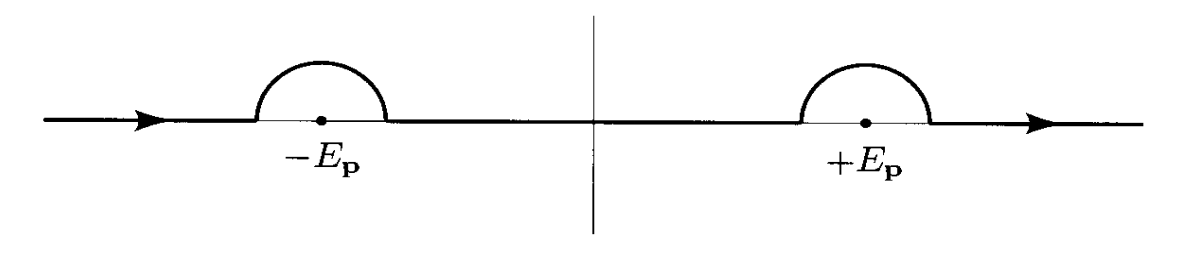
\includegraphics[height=3cm ,width=14cm]{./pic/R_Green.png}
\caption{Retarded Green Function}
\end{figure}
\[(\partial^2-m^2) D_R(x-y) = i \delta(x-y)\]
\[D_F(x-y) \equiv \langle 0 | T\phi(x) \phi(y) | 0 \rangle = \int \frac{d^4 p}{(2\pi)^4} \frac{-i}{p^2+m^2-i\epsilon} e^{ip(x-y)}\]
Here, $T$ stands for time ordering, placing all operators evaluated at later times to the left.
\begin{figure}[!h]
\centering
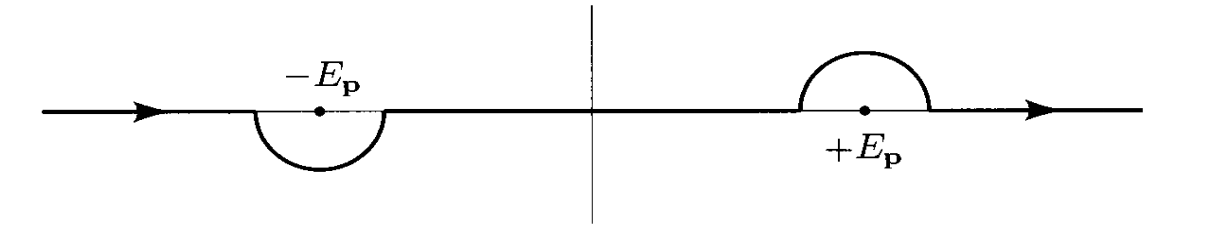
\includegraphics[height=3cm ,width=14cm]{./pic/F_Green.png}
\caption{Feynman Green Function}
\end{figure}

\subsection{Perturbation theory for canonical quantization}
\[\mathcal{L} = -\frac{1}{2}\partial_{\mu} \phi \partial^{\mu} \phi -\frac{1}{2}m_0^2 \phi^2 -\frac{\lambda_0}{4!}\phi^4\]
\[H = H_0 + H_{int} \quad H_{int} = \int d^3 x \frac{\lambda_0^4}{4!} \phi^4 (\vec{x})\]

\subsubsection{Perturbation expansion of correlation functions}
\paragraph{Note} The ground state of the interaction field theory is denoted by $| \Omega \rangle$, the ground state of the free field theory is denoted by $| 0 \rangle$. The zero of energy is defined by $H_0 | 0 \rangle =0$ and $E_0 = \langle \Omega | H | \Omega \rangle$.\\
\[\phi(t_0,\vec{x}) = \int \frac{d^3p}{(2\pi)^3}( a(\vec{p})e^{i\vec{p}\cdot\vec{x}} + a^{\dagger}(\vec{p})e^{-i\vec{p}\cdot\vec{x}})\]
\[\phi(t,\vec{x}) = e^{iH(t-t_0)} \phi(t_0,\vec{x}) e^{-iH(t-t_0)}\]
\[\phi_I(t,\vec{x}) \equiv e^{iH_0(t-t_0)} \phi(t_0,\vec{x}) e^{-iH_0(t-t_0)}\]
\[H_I(x) = \int d^3x \frac{\lambda_0^4}{4!} \phi_I^4\]
The perturbation expansion of correlation functions is
\[\langle \Omega | T \{ \phi(x) \phi(y) \} | \Omega \rangle = \lim_{T \to \infty(1-i\epsilon)} \frac{\langle 0 | T \left\{ \phi_I(x) \phi_I(y) \mathrm{exp} \left[ -i \int_{-T}^{T} dt H_I \right]\right\} | 0 \rangle}{\langle 0 | T \left\{ \mathrm{exp} \left[ -i \int_{-T}^{T} dt H_I \right]\right\} | 0 \rangle}\]
The proof can be found in chapter 4.2 of \emph{An introduction to quantum field theory (M.E.Peskin \& D.V.Schroeder)}

\subsubsection{Wick's theorem}
\[T \left\{ \phi(x_1) \phi(x_2) \cdots \phi(x_n)\right\} = N \left\{ \phi(x_1) \phi(x_2) \cdots \phi(x_n) + \mbox{ all possible contractions }\right\} \]
Normal order : all the $a$'s are to the right of all the $a^{\dagger}$.
\paragraph{Example} 
\begin{eqnarray}
\langle 0 | T \left\{ \phi_I(x_1) \phi_I(x_2) \phi_I(x_3) \phi_I(x_4)\right\}| 0 \rangle &=& D_F(x_1-x_2)D_F(x_3-x_4) \nonumber \\
&=& D_F(x_1-x_3)D_F(x_2-x_4) \nonumber \\
&=& D_F(x_1-x_4)D_F(x_2-x_3) \nonumber
\end{eqnarray}

\subsubsection{Feynman diagram}
Expand $\langle 0 | T \left\{ \phi_I(x) \phi_I(y) \mathrm{exp} \left[ -i \int_{-T}^{T} dt H_I \right]\right\} | 0 \rangle$ to the first order of $\lambda_0$
\begin{eqnarray}
& &\langle 0 | T \left\{ \phi_I(x) \phi_I(y) \frac{-i\lambda_0}{4!} \int dz^4 \phi_I(z) \phi_I(z) \phi_I(z) \phi_I(z) \right\} | 0 \rangle \nonumber \\
&=& 3 \cdot (\frac{-i\lambda_0}{4!}) D_F(x-y) \int d^4 z D_F(z-z) D_F(z-z) \nonumber \\
&+& 12 \cdot (\frac{-i\lambda_0}{4!}) \int d^4 z  D_F(x-z) D_F(y-z) D_F(z-z) \nonumber
\end{eqnarray}
It can be represented by the so called Feynman diagram.
\begin{figure}[!h]
\centering
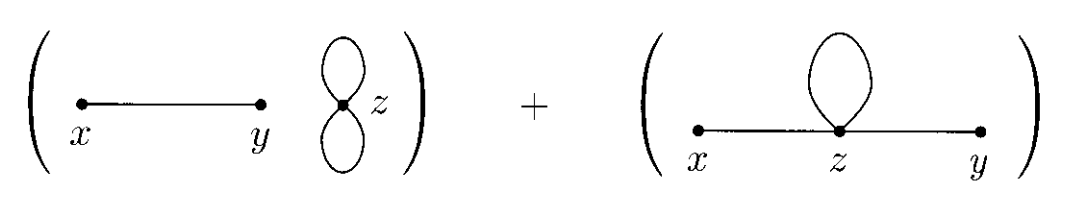
\includegraphics[height=1.5cm ,width=10cm]{./pic/FD1.png}
\caption*{}
\end{figure}
\\
The symmetry factor of the first diagram is $S = \frac{4!}{3} = 8$.
The symmetry factor of the second diagram is $S = \frac{4!}{12} = 2$.
The Feynman rules for $\phi^4$ theory are:\\
(1) For each propagator, $P = D_F(x-y)$;\\
(2) For each vertex, $V = (-i\lambda_0)\int d^4z$;\\
(3) For each external point, $E=1$;\\
(4) Divided by the symmetry factor.\\
At last, we can prove that
\[\langle \Omega | T \{ \phi_I(x_1) \phi_I(x_2) \cdots \phi_I(x_n) \} | \Omega \rangle = \mbox{ sum of all E-connected diagrams with n external points}\]
Here, the "E-disconnected" means disconnected from all external points", being called "vacuum bubbles". They vacuum bubbles in $\langle 0 | T \left\{ \phi_I(x_1) \phi_I(x_2) \cdots \phi_I(x_n) \mathrm{exp} \left[ -i \int_{-T}^{T} dt H_I \right]\right\} | 0 \rangle$ are all cancelled by the $\langle 0 | T \left\{ \mathrm{exp} \left[ -i \int_{-T}^{T} dt H_I \right]\right\} | 0 \rangle$.

\subsection{Path integral formulation}
\subsubsection{Basic equation}
Recall the path integrals in quantum mechanics, we abandon the Hamiltonian formalism and define the Hamiltonian dynamics as
\[\langle \phi_b(\vec{x}) | e^{-iHT} | \phi_a(\vec{x}) \rangle = \int \mathcal{D}\phi  \mathrm{exp} \left[ i\int_0^T d^4x \mathcal{L} \right]\]
Here, $\langle \phi_b(\vec{x}) |$ is the eigenstate of $\phi_S(\vec{x})=\phi_H(\vec{x},0)$ with eigenvalue $\phi_b(\vec{x})$ at time $t=T$,$| \phi_a(\vec{x}) \rangle$ is the eigenstate of $\phi_S(\vec{x})$ with eigenvalue $\phi_a(\vec{x})$ at time $t=0$.\\
We emphasize that in this subsection, $\phi_H$ denotes the Heisenberg picture of field whose value is operators,$\phi_S$ denotes the Schr\"{o}dinger picture of field, $\phi(x)$ is classical field whose value is ordinary number.

\subsubsection{Correlation function}
\[\langle \Omega | T \phi_H(x_1) \phi_H(x_2)| \Omega \rangle = \lim_{T \to \infty(1-i\epsilon)} \frac{\int \mathcal{D}\phi \phi(x_1)\phi(x_2) \mathrm{exp} \left[ i\int_T^T d^4x \mathcal{L} \right]}{\int \mathcal{D} \phi \mathrm{exp} \left[ i\int_T^T d^4x \mathcal{L} \right]}\]
The proof can be found in chapter 9.2 of \emph{An introduction to quantum field theory (M.E.Peskin \& D.V.Schroeder)}.

\subsubsection{Functional derivatives and the generating functional}
We define the generating functional as
\[Z[J] \equiv \int \mathcal{D} \phi \mathrm{exp} \left[ i\int d^4x \mathcal{L} + J(x)\phi(x) \right]\]
We can prove that
\[\langle \Omega | T \phi_H(x_1) \cdots \phi_H(x_n) | \Omega \rangle = \frac{1}{Z_0} \left( -i\frac{\delta}{\delta J(x_1)} \right)\cdots \left( -i\frac{\delta}{\delta J(x_n)} \right) Z[J]|_{J=0}\]
Here, $Z_0 \equiv Z[J=0]$.

\subsubsection{Free field theory}
In Klein-Gordon field theory,
\[\int d^4x [\mathcal{L}_0(\phi)+J\phi] = \int d^4x [\frac{1}{2}\phi (\partial^2 -m^2+i\epsilon)\phi + J\phi]\]
Define
\[\phi'(x) \equiv \phi(x) + \int d^4y (-iD_F(x-y)) J(y) \]
Recall that $(\partial^2-m^2)D_F(x-y) = i\delta(x-y)$, we can derive that
\[\int d^4x [\mathcal{L}_0+J\phi] = \int d^4x [\frac{1}{2}\phi' (\partial^2 -m^2+i\epsilon)\phi'] - \int d^4x d^4y \frac{1}{2} J(x)[-iD_F(x-y)]J(y)\]
After integration, we can know that
\[Z[J] = Z_0 \mathrm{exp} [-\frac{1}{2} \int d^4x d^4y J(x)D_F(x-y)J(y)]\]
So,
\[\langle 0 | T \phi_H(x_1) \phi_H(x_2) | 0 \rangle =  - \frac{\delta}{\delta J(x_1)} \frac{\delta}{\delta J(x_2)} \mathrm{exp} [-\frac{1}{2} \int d^4x d^4y J(x)D_F(x-y)J(y)]|_{J=0} = D_F(x_1-x_2)\]

\subsection{Perturbation theory for path integral quantization}
\begin{eqnarray}
\mathcal{L} &=& -\frac{1}{2}\partial_{\mu} \phi \partial^{\mu} \phi -\frac{1}{2}m_0^2 \phi^2 -\frac{\lambda_0}{4!}\phi^4 \quad \mathcal{L} = \mathcal{L}_0 + \mathcal{L}_1 \quad \mathcal{L}_1 =- \frac{\lambda_0}{4!} \phi^4 (\vec{x}) \nonumber \\
Z[J] &=& \int \mathcal{D}\phi e^{i\int d^4x [\mathcal{L}_0 + \mathcal{L}_1 + J\phi]} \nonumber \\
&=& e^{i\int d^4y \mathcal{L}_1(\frac{1}{i} \frac{\delta}{\delta J(y)})} \int \mathcal{D}\phi e^{i\int d^4x [\mathcal{L}_0 + J\phi]} \nonumber \\
&\propto & e^{i\int d^4x \mathcal{L}_1(\frac{1}{i} \frac{\delta}{\delta J(x)})} \mathrm{exp} [-\frac{1}{2} \int d^4y d^4z J(y)D_F(y-z)J(z)] \nonumber \\
& =& \sum_{V=0}^{\infty} \frac{1}{V!} [ \frac{-i\lambda_0}{4!} \int d^4x (\frac{1}{i} \frac{\delta}{\delta J(x)})^4]^V \times \sum_{P=0}^{\infty} \frac{1}{P!} [-\frac{1}{2} \int d^4y d^4z J(y)D_F(y-z)J(z)]^P
\end{eqnarray}
If we focus on a term with particular values of V and P, then
the number of surviving sources (after we take all the functional derivatives) is $E = 2P-4V$. The $4V$ functional derivatives can act on the 2P sources in $\frac{(2P)!}{(2P-4V)!}$ different combinations. However, many of the resulting expressions are algebraically identical.\\
To organize them, we introduce Feynman diagrams similar to that in perturbation theory of canonical quantization. In these diagrams, a line segment stands for a propagator $D_F(x-y)$, a filled circle at one end of a line segment for a source $i\int d^4x J(x)$, and a vertex joining four line segments for $-i\lambda_0 \int d^4 z$.\\
For each diagram, we can assign a symmetry factor $S_P$ similar to that in perturbation theory for canonical quantization. Due to the fact that some external sources are identical here, usually $S_P \neq S_C$. But when calculating the correlation function, the exchange of the order of functional derivatives to identical sources can eliminate the difference.\\
We can demonstrate that
\[Z[J] \propto \mathrm{exp}(\sum_I C_I)\]
Here, $C_I$ stands for a particular connected diagram, including its symmetry factor. We define $W[J]$ as
\[Z[J] \equiv Z_0 \mathrm{exp}(-iW[J])\]
As, $W[0]=0$, we know
\[-iW[J] = \sum_{I \neq \{0\}} C_I\]
The notation $I\neq \{0\}$ means that the vacuum diagrams are omitted from the sum.\\
The detailed discussion can be found in chapter 9 of \emph{Quantum field theory (M. Srednicki)}.

\subsection{LSZ reduction formula}
\subsubsection{Field strength renormalization}
The completeness relation:
\[\mathbf{1} = |\Omega\rangle\langle\Omega| +  \sum_{\lambda} \int \frac{d^3p}{(2\pi)^3} \frac{1}{2E_{\mathbf{p}}} |\lambda_{\mathbf{p}}\rangle\langle\lambda_{\mathbf{p}}|\]
Here, $E_{\mathbf{p}} = \sqrt{m_{\lambda}^2 + \mathbf{p}^2}$\\
\begin{figure}[!h]
\centering
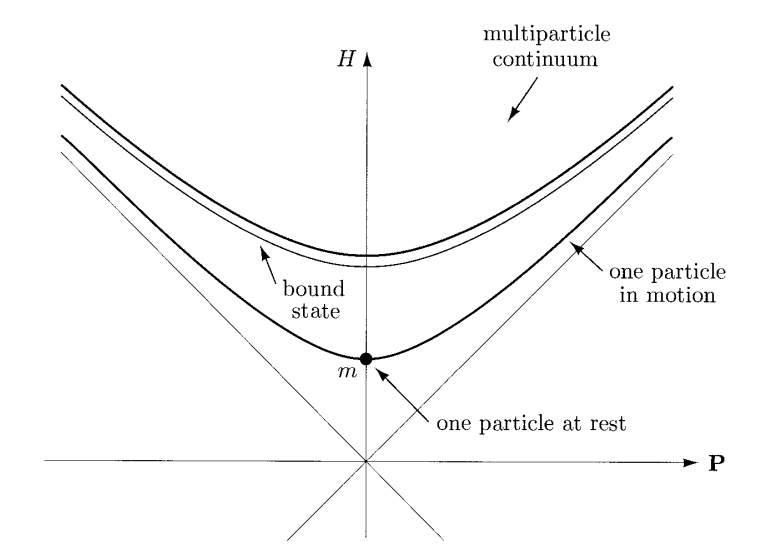
\includegraphics[height=7cm ,width=12cm]{./pic/FSR1.png}
\caption*{}
\end{figure}
\\
Assume for now $x^0 > y^0$ and define $\langle \Omega | \phi(x) \phi(y) | \Omega \rangle_{C} = \langle \Omega | \phi(x) \phi(y) | \Omega \rangle - \langle \Omega | \phi(x)| \Omega \rangle \langle | \Omega \phi(y) | \Omega \rangle$ as connected two point function. (The term $\langle \Omega | \phi(x)| \Omega \rangle \langle | \Omega \phi(y) | \Omega \rangle$ is usually zero by symmetry; for higher spin fields, it is zero by Lorentz invariance.) The connected two point function is
\[\langle \Omega | \phi(x) \phi(y) | \Omega \rangle_{C} = \sum_{\lambda} \int \frac{d^3p}{(2\pi)^3} \frac{1}{2E_{\mathbf{p}}} \langle \Omega | \phi(x) |\lambda_{\mathbf{p}}\rangle\langle\lambda_{\mathbf{p}}| \phi(y) | \Omega \rangle\]
It can be verified that
\[\langle \Omega | \phi(x) |\lambda_{\mathbf{p}}\rangle = \langle \langle \Omega | \phi(0) | \lambda_0 \rangle e^{ipx} |_{p^0 = E_{\mathbf{p}}}\]
So,
\[\langle \Omega | \phi(x) \phi(y) | \Omega \rangle_C = \sum_{\lambda} \int \frac{d^4p}{(2\pi)^4} \frac{-i}{p^2 + m_{\lambda}^2 -i\epsilon} e^{ip(x-y)} |\langle \Omega | \phi(0) | \lambda_0 \rangle|^2\]
Analogous expressions hold for the case $y^0 > x^0$, and both cases can be summarized as
\[\langle \Omega | T \phi(x) \phi(y) | \Omega \rangle_C = \int_0^{\infty} \frac{dM^2}{2\pi} \rho(M^2) D_F(x-y;M^2)\]
and 
\[\rho(M^2) = \sum_{\lambda} (2\pi) \delta(M^2-m^2)|\langle \Omega | \phi(0) | \lambda_0 \rangle|^2 \]
\begin{figure}[!h]
\centering
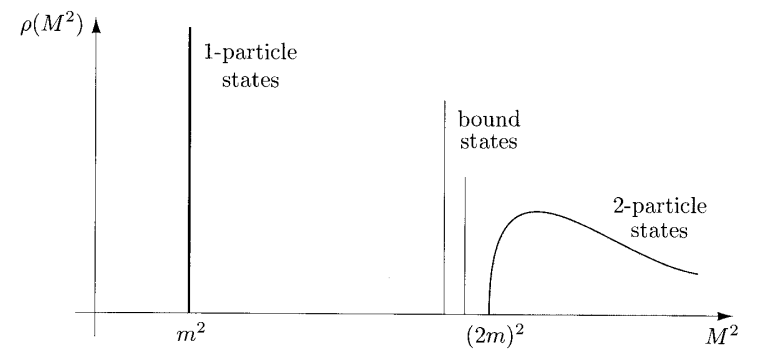
\includegraphics[height=5cm ,width=12cm]{./pic/FSR2.png}
\caption*{The structure of the spectral density function $\rho(M^2)$}
\end{figure}\\
The one-particle state contribute an isolated delta function to the spectral density function, so
\[\rho(M^2) = 2\pi \delta (M^2 -m^2) \cdot Z + \mbox{ (nothing else until $M^2 > \sim (2m)^2$) }\]
$Z = |\langle \Omega | \phi(0) | \lambda_0 \rangle|^2$ is called field-strength renormalization. $m$ is the physical mass of a single particle of the $\phi$ boson. The Fourier transformation of the two point function is
\[\int d^4x e^{-ipx} \langle \Omega | T \phi(x) \phi(0) | \Omega \rangle_C  = \int_{0}^{\infty} \frac{dM^2}{2\pi} \rho(M^2) \frac{-i}{p^2+M^2-i\epsilon} = \frac{-iZ}{p^2+m^2-i\epsilon} +  \int_{\sim 4m^2}^{\infty} \frac{dM^2}{2\pi} \rho(M^2) \frac{-i}{p^2+M^2-i\epsilon}\]
\begin{figure}[!h]
\centering
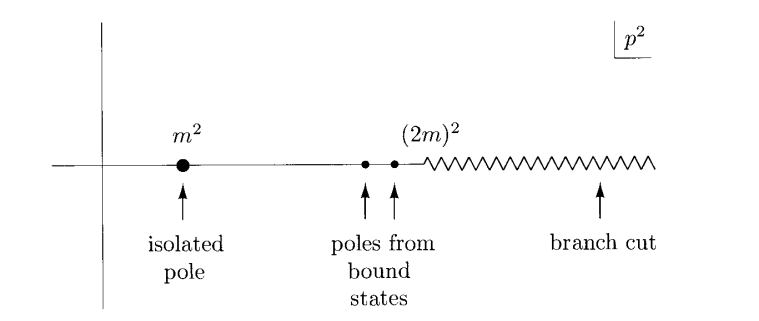
\includegraphics[height=4cm ,width=12cm]{./pic/FSR3.png}
\caption*{The structure of the two point function in Fourier space}
\end{figure}\\
\subsubsection{LSZ reduction formula}
\begin{eqnarray}
&& \quad \prod_1^n \int d^4 x_i e^{-ip_ix_i} \prod_1^m d^4 y_i e^{ik_jy_j} \langle \omega | T \{\phi(x_1) \cdots \phi(x_n) \phi(y_1) \cdots \phi(y_m)\} | \Omega \rangle \nonumber \\
&& \underset{ p_i^0 \to E_{\mathbf{p}_i}\, k_i^0 \to E_{\mathbf{k}_i}}{\sim}  \left( \prod_1^n \frac{-\sqrt{Z} i}{p_i^2 + m^2 -i\epsilon} \right) \left( \prod_1^m \frac{-\sqrt{Z} i}{k_i^2 + m^2 -i\epsilon} \right) \langle \mathbf{p}_1 \cdots \mathbf{p}_n | S | \mathbf{k}_1 \cdots \mathbf{k}_m \rangle \nonumber
\end{eqnarray}
The $\sim$ means the two sides of the expression share the same singular structure around $p_i^0 \to E_{\mathbf{p}_i}$, $k_i^0 \to E_{\mathbf{k}_i}$.
The proof can be found in chapter 7.2 of \emph{An introduction to quantum field theory (M.E.Peskin \& D.V.Schroeder)}.
To express the formula above in the language of Feynman diagrams, we consider the S-matrix element for 2-particle $\to$ 2-particle for example. Note the disconnected diagram should be disregarded because they do not have the singularity structure with a product of four poles indicated by on the right side of the LSZ reduction formula. So, the exact four point function
\[\prod_1^2 \int d^4 x_i e^{-ip_ix_i} \prod_1^2 d^4 y_i e^{ik_jy_j} \langle \omega | T \{\phi(x_1)\phi(x_2)\phi(y_1) \phi(y_2)\} | \Omega \rangle \]
has the general form showed as below.
\begin{figure}[!h]
\centering
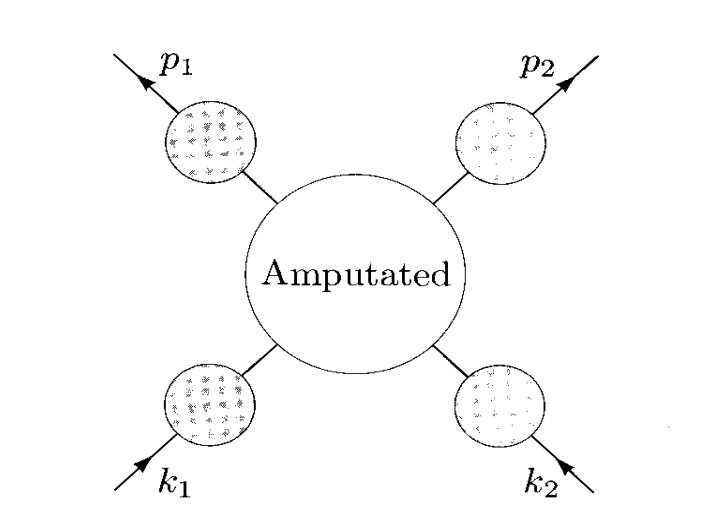
\includegraphics[height=4cm ,width=5cm]{./pic/LSZ1.png}
\caption*{}
\end{figure}\\
\paragraph{Note} One-particle-irreducible, or 1PI for short, refers to diagrams that is still connected after one line is cut.\\ 
We can sum up the corrections to each external leg. Let $-iM^2(p^2)$ denote the sum of all 1PI insertions into the scalar propagator:
\begin{figure}[!h]
\centering
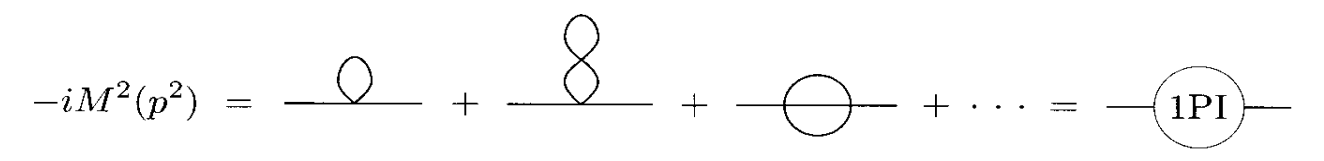
\includegraphics[height=2cm ,width=15cm]{./pic/LSZ2.png}
\caption*{}
\end{figure}\\
Then the exact propagator can be written as a geometric series as
\begin{figure}[!h]
\centering
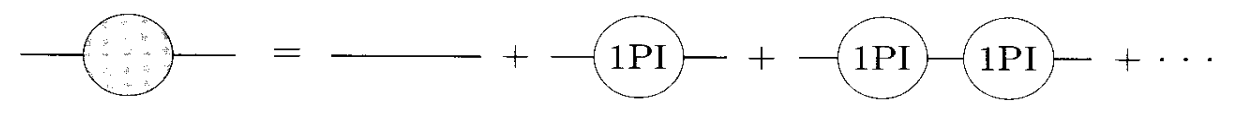
\includegraphics[height=1.5cm ,width=15cm]{./pic/LSZ3.png}
\caption*{}
\end{figure}\\
The result is $\frac{-i}{p^2 + m_0^2 + M^2}$. If we expand each resummed propagator about the physical particle pole, we see that each external leg of the four-point amplitude contributes
\[\frac{-i}{p^2 + m_0^2 + M^2} \underset{p^0 \to E_{\mathbf{p}}}{\sim} \frac{-iZ}{p^2+m^2} + \mbox{ (regular) }\]
Thus, the sum of diagrams contains a product of four point poles:
\[\frac{-iZ}{p_1^2 + m^2} \frac{-iZ}{p_2^2 + m^2} \frac{-iZ}{k_1^2 + m^2} \frac{-iZ}{k_2^2 + m^2}\]
So, the S matrix element can be represented by 
\begin{figure}[!h]
\centering
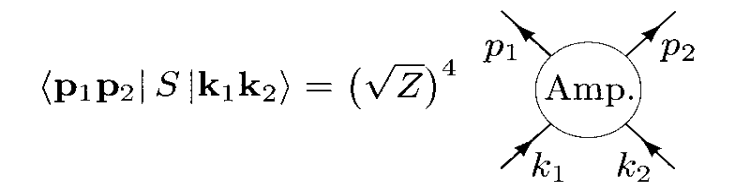
\includegraphics[height=2cm ,width=8cm]{./pic/LSZ4.png}
\caption*{}
\end{figure}\\
It is easy to be generalized to the more complicated scattering cases. After Fourier transforming the n-point function to momentum space and cutting off the external legs, the Feynman rules for S-matrix element can be stated as follows:\\
(1) For each propagator, $P = \frac{-i}{p^2 + m_0^2 -i\epsilon}$;\\
(2) For each vertex, $V = -i\lambda_0$;\\
(3) For each external point, $E=1$;\\
(4) Impose momentum conservation at each vertex;\\
(5) Integrate over each undetermined loop momentum: $\int \frac{d^4p}{(2\pi)^4}$;\\
(6) Divided by the symmetry factor;\\
(7) Multiply the total momentum conservation factor $(2\pi)^4 \delta(\sum p_f - \sum p_i)$ 
We can write $\langle f | S | i \rangle = i \mathcal{M} (2\pi)^4 \delta(\sum p_f - \sum p_i)$ for convenience.

\subsection{Re-normalization}
Re-normalization, the procedure in quantum field theory by which divergent parts of a calculation, leading to nonsensical infinite results, are absorbed by redefinition into a few measurable quantities, so yielding finite answers.
\subsubsection{Counting of ultraviolet divergence}
Consider a pure scalar theory in $d$ dimensions with a $\phi^n$ interaction term
\[\mathcal{L} = -\frac{1}{2} \partial^{\mu} \phi \partial_{\mu} \phi -\frac{1}{2}m^2 \phi^2 - \frac{\lambda}{n!}\phi^n\]
Let $N$ be the number of external lines in the diagram, $P$ the number of propagators, $V$ the number of vertices. The number of the loops in the diagram is $L=P-V+1$.  There are $n$ lines meeting at each vertex, so $nV = 2P+N$. Loosely speaking, each loop has an integral $d^d p$, each propagator has a factor $p^{-2}$, so the superficial degrees of divergence is
\[D = dL - 2P = d + [n(\frac{d-2}{2})-d)]V - (\frac{d-2}{2})N\]
According the superficial degrees of divergence of the diagram. These three possible types of ultraviolet behaviour of quantum field theories. We will refer to them as follows:\\
(1) Super-Re-normalizable theory: Only a finite number of Feynman diagrams superficially diverge.\\
(2) Re-normalizable theory: Only a finite number of amplitudes superficially diverge; however, divergences
occur at all orders in perturbation theory. \\
(3) Non-Re-normalizable theory: All amplitudes are divergent at a sufficiently high order in perturbation
theory.\\
So, for $\phi^4$ theory in four dimension, $D = 4 - N$. It is a re-normalizable theory. For $\phi^3$ theory in four dimension, $D = 4 - V -N$. It is a super-re-normalizable theory. For $\phi^6$ theory in four dimension, $D = 4 + 2V -N$. It is a Non-re-normalizable theory. \\
The superficial degrees of freedom can also be derived from dimensional analysis. The dimension of $\lambda$ is $d - \frac{n(d-2)}{2}$. Now consider an arbitrary diagram with $N$ external lines. One way that such a diagram could arise is from an interaction term $\eta \phi^N$ in the Lagrangian. The dimension of $\eta$ would then be $d - \frac{N(d-2)}{2}$, and therefore we conclude that any (amputated) diagram with $N$ external lines has dimension $d - \frac{N(d-2)}{2}$. In our theory with only the $\lambda \phi^n$ vertex, if the diagram has $V$ vertices, its divergent part is proportional to $\lambda^V \Lambda^D$, where $\Lambda$ is a high momentum cut-off and $D$ is the superficial degree of divergence.  Applying dimensional analysis, we find
\[d - \frac{N(d-2)}{2} = V[d - \frac{n(d-2)}{2}] + D\]
Note that the quantity that multiplies $V$ in this expression is just the dimension of the coupling constant $\lambda$. Thus we can characterize the three degrees of re-normalizability in a second way:\\
(1) Super-Re-normalizable: Coupling constant has positive mass dimension.\\
(2) Re-normalizable: Coupling constant is dimensionless.\\
(3) Non-Re-normalizable: Coupling constant has negative mass dimension.

\subsubsection{Renormalized Perturbation Theory}
The Lagrangian of $\phi^4$ theory is 
\[\mathcal{L} = -\frac{1}{2} \partial^{\mu} \phi \partial_{\mu} \phi -\frac{1}{2}m_0^2 \phi^2 - \frac{\lambda_0}{4!}\phi^4\]
We write $m_0$ and $\lambda_0$, to emphasize that these are the bare values of the mass and coupling constant, not the values measured in experiments.
Since the theory is invariant under $\phi \to -\phi$, all amplitudes with an odd number of external legs vanish. The only divergent amplitudes are therefore
\begin{figure}[!h]
\centering
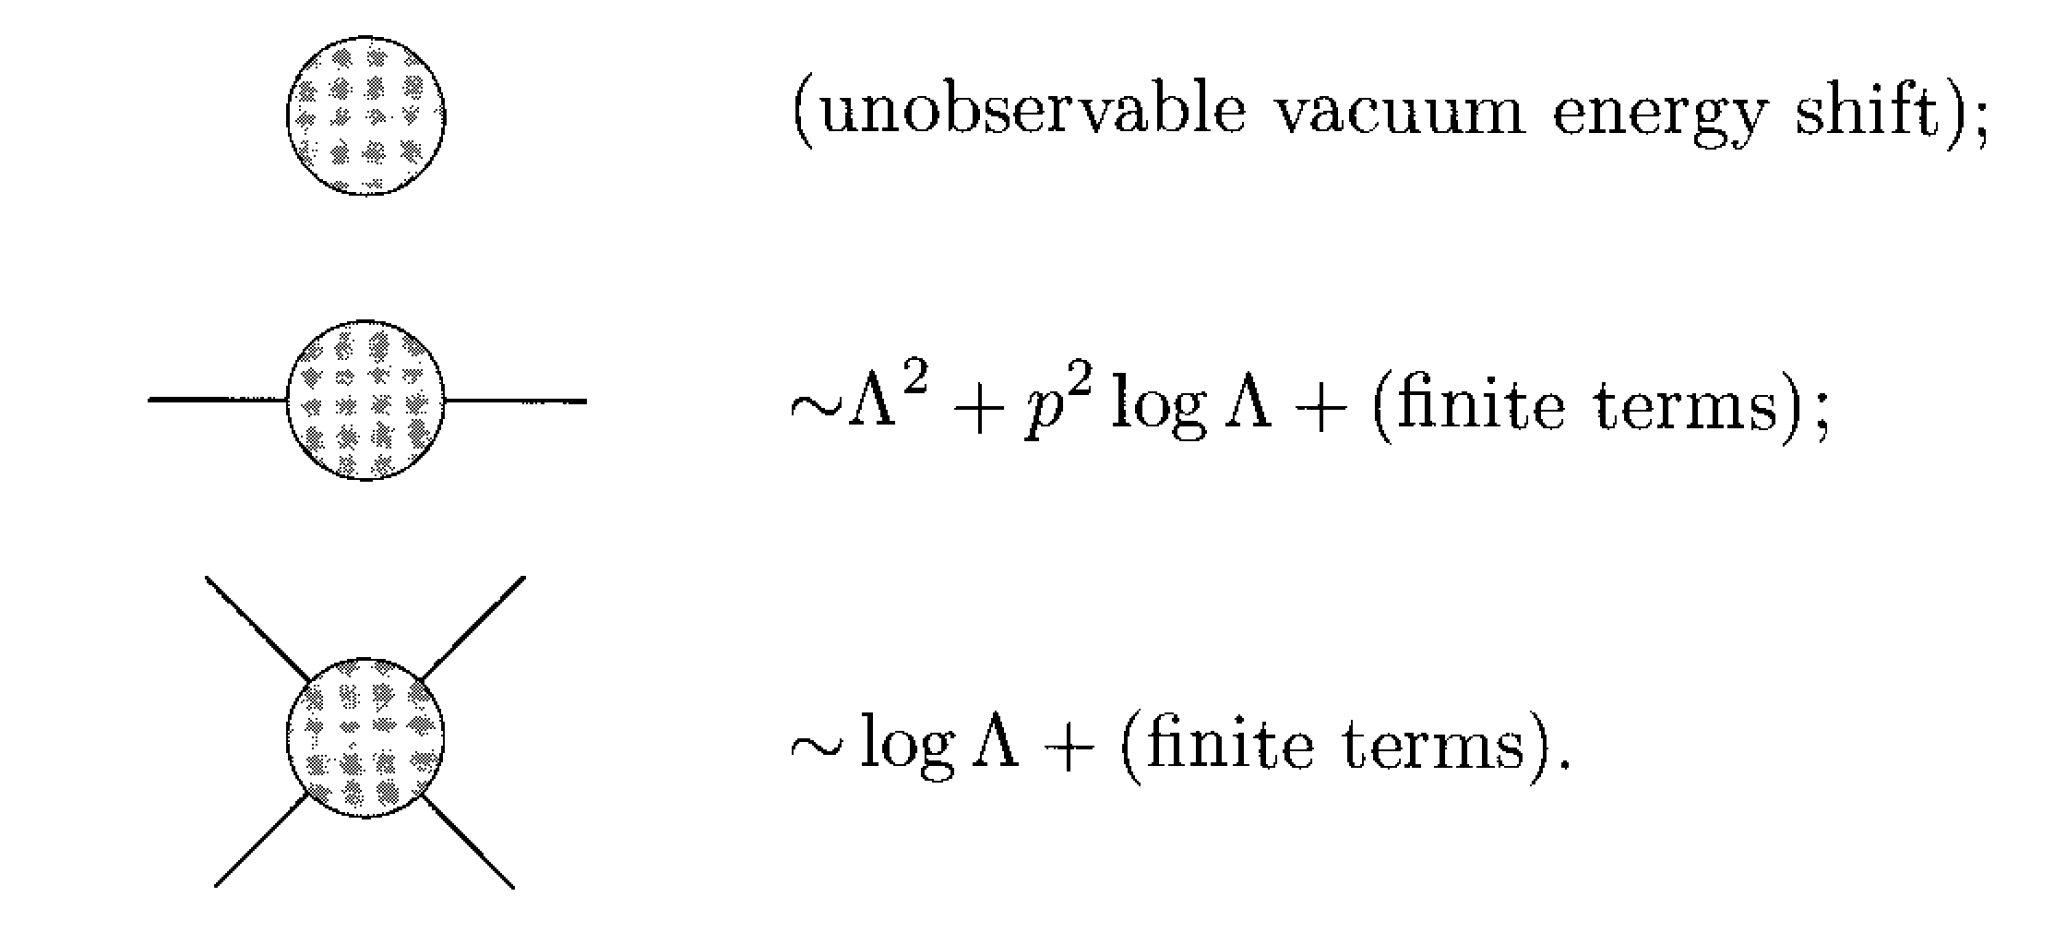
\includegraphics[height=4cm ,width=9cm]{./pic/RG1.png}
\caption*{}
\end{figure}\\
Ignoring the vacuum diagram, these amplitudes contain three infinite constants. Our goal is to absorb these constants into the three unobservable parameters of the theory: the bare mass, the bare coupling constant, and the field strength. To accomplish this goal, it is convenient to reformulate the perturbation expansion so that these unobservable quantities do not appear
explicitly in the Feynman rules. Recall that the exact two-point function has the form
\[\int d^4x \langle \Omega | \phi(x) \phi(0) | \Omega \rangle e^{-ipx} = \frac{-iZ}{p^2+m^2} + \mbox{ terms regular at } p^2 = m^2\]
We can eliminate the $Z$ from this equation by rescaling the field:
$\phi = Z^{\frac{1}{2}} \phi_r$
We also define
\[\delta_Z = Z -1 \quad \delta_m = Zm_0^2 - m^2 \quad \delta_{\lambda} = \lambda_0 Z^2 - \lambda\]
Then the Lagrangian becomes
\[\mathcal{L} = -\frac{1}{2} \partial^{\mu} \phi_r \partial_{\mu} \phi_r -\frac{1}{2}m^2 \phi_r^2 - \frac{\lambda}{4!}\phi_r^4 -\frac{1}{2} \delta_Z \partial^{\mu} \phi_r \partial_{\mu} \phi_r -\frac{1}{2}\delta_m \phi_r^2 - \frac{\delta \lambda}{4!}\phi_r^4\]
The last three terms, known as counter-terms, have absorbed the infinite but unobservable shifts between the bare parameters and the physical parameters.\\
We give precise definitions of the physical mass and coupling constant as follows. The re-normalization scheme here is called on-shell (OS) scheme. Other re-normalization scheme would be introduced later.\\
\begin{figure}[!h]
\centering
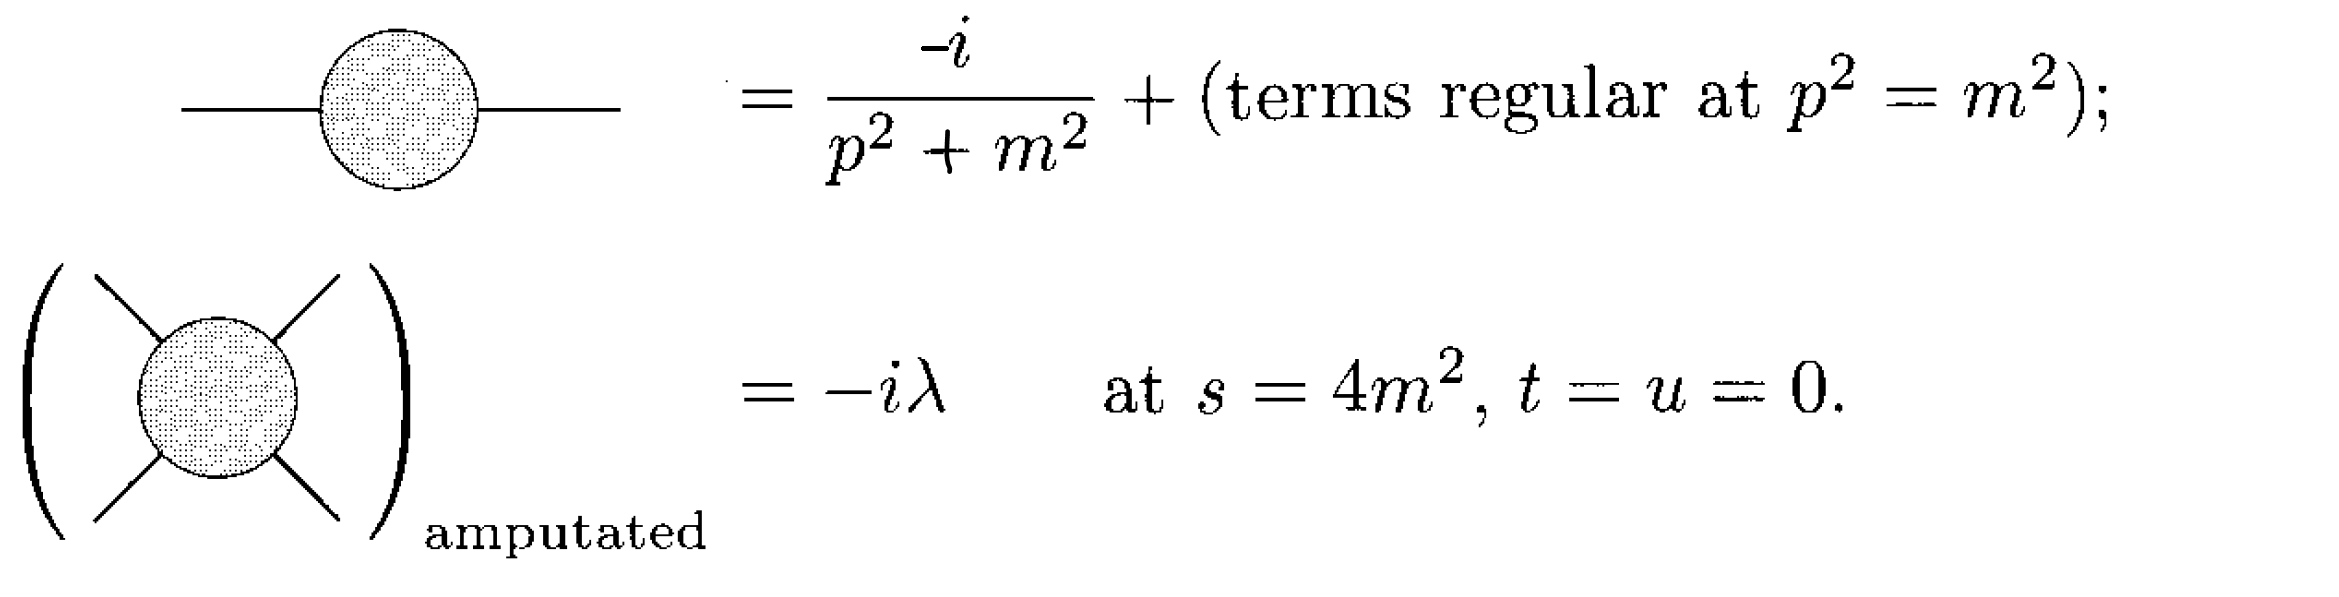
\includegraphics[height=3cm ,width=11cm]{./pic/RG2.png}
\caption*{}
\end{figure}\\
These equations are called re-normalization conditions.
Our new Lagrangian gives a new set of Feynman rules,\\
\begin{figure}[!h]
\centering
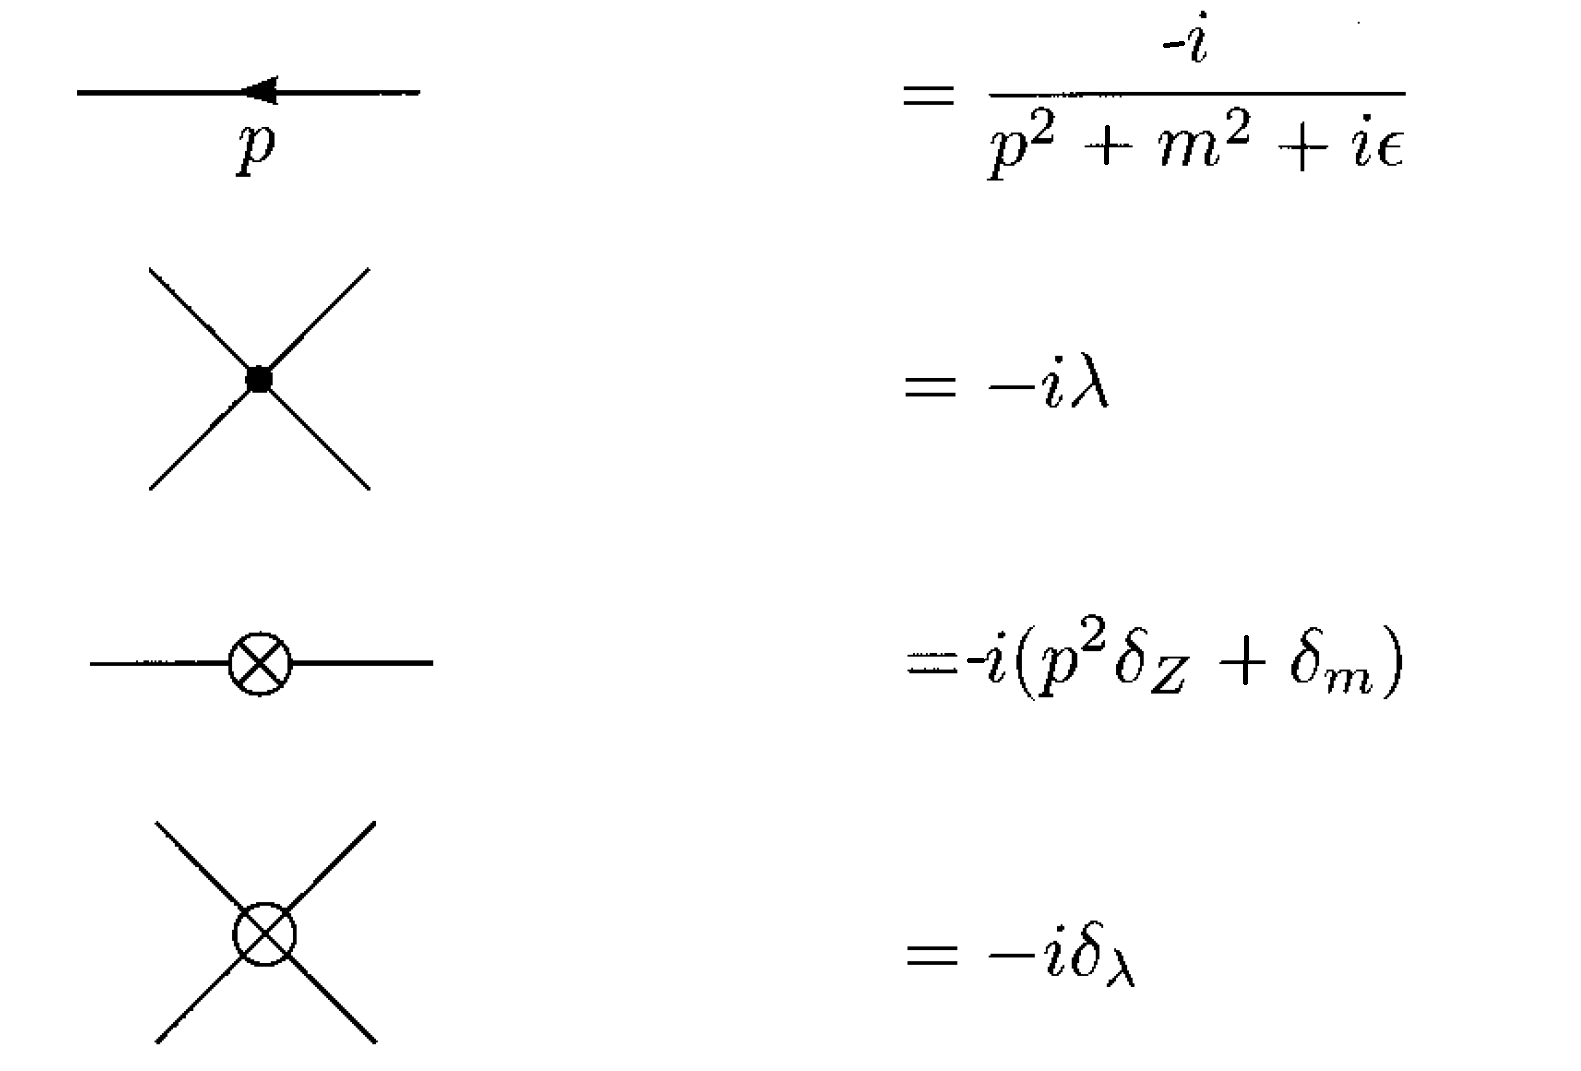
\includegraphics[height=6cm ,width=9cm]{./pic/RG3.png}
\caption*{}
\end{figure}\\
We can use these new Feynman rules to compute any amplitude in $\phi^4$ theory. The procedure is as follows. Compute the desired amplitude as the sum of all possible diagrams created from the propagator and vertices shown above. The loop integrals in the diagrams will often diverge, so one must introduce a regulator. The result of this computation will be a function of the three unknown parameters $\delta_Z$, $\delta_m$, and $\delta_{\lambda}$. Adjust ( or "renormalise") these three parameters as necessary to maintain the re-normalization conditions. After this adjustment, the expression for the amplitude should be finite and independent of the regulator. \\
This procedure, using Feynman rules with counter-terms, is known as renormalized perturbation theory. 

\subsubsection{Mandelstam variable}
In theoretical physics, the \href{https://en.wikipedia.org/wiki/Mandelstam_variables}{\textbf{Mandelstam variable}}  are numerical quantities that encode the energy, momentum, and angles of particles in a scattering process in a Lorentz-invariant fashion. They are used for scattering processes of two particles to two particles. 
The Mandelstam variables $s$, $t$, $u$ are then defined by
\begin{eqnarray}
s=-(p_{1}+p_{2})^{2}=-(p_{3}+p_{4})^{2} \nonumber \\
t=-(p_{1}-p_{3})^{2}=-(p_{2}-p_{4})^{2} \nonumber \\
u=-(p_{1}-p_{4})^{2}=-(p_{2}-p_{3})^{2} \nonumber
\end{eqnarray}
Where $p_1$ and $p_2$ are the four-momenta of the incoming particles and $p_3$ and $p_4$ are the four-momenta of the outgoing particles.
$s$ is also known as the square of the center-of-mass energy (invariant mass) and $t$ is also known as the square of the four-momentum transfer.\\
We can verify that
\[s+t+u = m_1^2 + m_3^2 + m_3^2 +m_4^2\]

\subsubsection{Feynman's formula}
\[ \frac{1}{A_1 \cdots A_n} = \int dF_n (x_1A_1+ \cdots +x_nA_n)^{-n}\]
where the integration measure over the Feynman parameters $x_i$ is
\[\int dF_n = (n-1)! \int_0^1 dx_1 \cdots dx_n \delta(x_1+\cdots+x_n-1)\]
This measure is normalized so that
\[\int dF_n = 1\]
A generalization of Feynman's formula is
\[ \frac{1}{A_1^{\alpha_1} \cdots A_n^{\alpha_n}} = \frac{\Gamma(\sum_i \alpha_i)}{\prod_i \Gamma(\alpha_i)} \frac{1}{(n-1)!}\int dF_n \frac{\prod_i x_i^{\alpha_i-1}}{(\sum_i x_i A_i)^{\sum_i \alpha_i}}\]

\begin{figure}[!h]
\centering
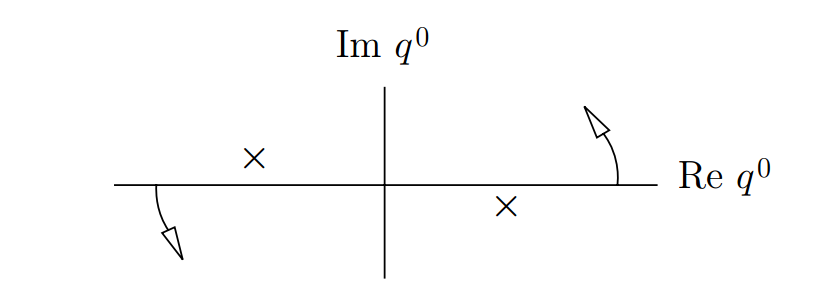
\includegraphics[height=3cm ,width=5cm]{./pic/RG5.png}
\caption*{Wick rotation}
\end{figure}
\subsubsection{Wick rotation}
For an integral $\int d^d q f(q^2-i\epsilon)$, if the integrand vanishes fast enough as $|q_0| \to \infty$, we can rotate this contour clockwise by $\frac{\pi}{2}$, so that it runs from $-i\infty$ to $i\infty$. In making this Wick rotation, the contour does not pass over any poles. (The $i\epsilon$ are needed to make this statement unambiguous.) Thus the value of the integral is unchanged. It is now convenient to define a Euclidean d-dimensional vector $\bar{q}$ via $q^0 = i \bar{q}_d$ and $q_j = \bar{q}_j$; then $q^2 = \bar{q}^2$, where
\[\bar{q}^2 = \bar{q}_1^2 + \cdots + \bar{q}_d^2\]
Also, $d^dq = id^d \bar{q}$.Therefore, in general,
\[\int d^d q f(q^2-i\epsilon) = i \int d^d\bar{q} f(\bar{q}^2)\]


\subsubsection{Dimensional regularization}
Dimensional regularization is a method for regularizing integrals in the evaluation of Feynman diagrams. For example, if one wishes to evaluate a loop integral which is logarithmically divergent in four dimensions, like
\[\int {\frac {d^{d}p}{(2\pi )^{d}}}{\frac {1}{\left(p^{2}+m^{2}\right)^{2}}}\]
one first rewrites the integral in some way so that the number of variables integrated over does not depend on d, and then we formally vary the parameter $d$, to include non-integral values like $d=4-\epsilon$.
\[\int _{0}^{\infty }{\frac {dp}{(2\pi )^{4-\varepsilon }}}{\frac {2\pi ^{(4-\varepsilon )/2}}{\Gamma \left({\frac {4-\varepsilon }{2}}\right)}}{\frac {p^{3-\varepsilon }}{\left(p^{2}+m^{2}\right)^{2}}}={\frac {2^{\varepsilon -4}\pi ^{{\frac {\varepsilon }{2}}-1}}{\sin({\frac {\pi \varepsilon }{2}})\Gamma (1-{\frac {\varepsilon }{2}})}}m^{-\varepsilon }={\frac {1}{8\pi ^{2}\varepsilon }}-{\frac {1}{16\pi ^{2}}}\left(\ln {\frac {m^{2}}{4\pi }}+\gamma \right)+{\mathcal {O}}(\varepsilon )\]
There is a useful formula for calculating the integral
\[\int \frac{d^d \bar{q}}{(2\pi)^{d}} \frac{(\bar{q}^2)^a}{(\bar{q}^2+D)^b} = \frac{\Gamma(b-a-\frac{1}{2}d) \Gamma(a+\frac{1}{2}d)}{(4\pi)^{d/2} \Gamma(b) \Gamma(\frac{1}{2}d)} D^{-(b-a-d/2)}\]
If $a=0$, then the formula will be
\[\int \frac{d^d \bar{q}}{(2\pi)^{d}} \frac{1}{(\bar{q}^2+D)^b} = \frac{\Gamma(b-\frac{1}{2}d)}{(4\pi)^{d/2} \Gamma(b)} D^{-(b-d/2)}\]

\subsubsection{One loop structure of $\phi^4$ theory}
First consider the basic two-particle scattering amplitude,
\begin{figure}[!h]
\centering
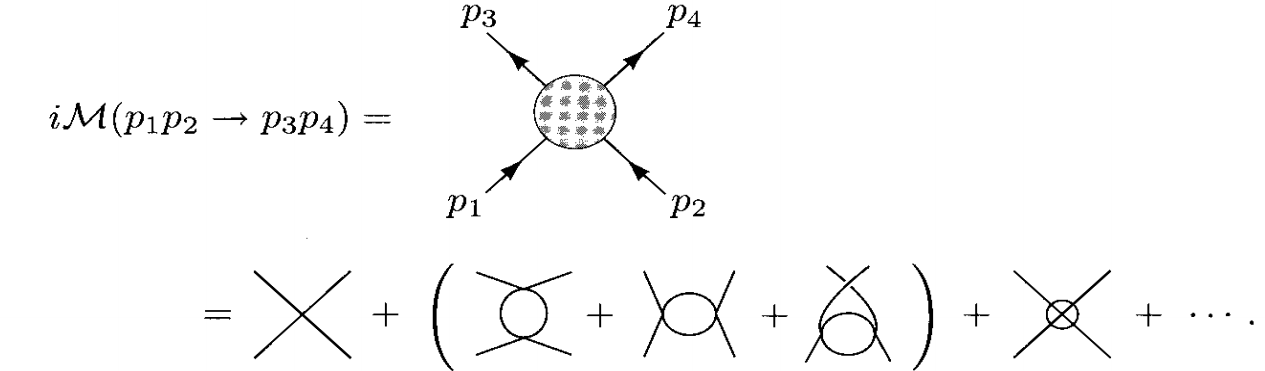
\includegraphics[height=3cm ,width=11cm]{./pic/RG4.png}
\caption*{}
\end{figure}\\
If we define $p = p_1 + p_2$, then the second diagram is
\[\frac{(-i\lambda)^2}{2} \int \frac{d^4k}{(2\pi)^4} \frac{-i}{k^2+m^2} \frac{-i}{(k+m)^2+m^2} \equiv (-i\lambda)^2 iV(-p^2)\]
So the entire amplitude is therefore
\[i\mathcal{M} = -i\lambda + (-i\lambda)^2 [iV(s) + iV(t) iV(u)] -i\delta_{\lambda} + \mathcal{O}(\lambda^3)\]
To keep $\lambda$ dimensionless in dimensional regularization, we can make the transformation $\lambda \to \lambda \tilde{\mu}^{\epsilon}$. Here, $\mu$ is an arbitrary number with mass dimension 1 and $\epsilon \equiv 4-d$. 
We can calculate that
\[V(-p^2) = -\frac{1}{32\pi^2} \int_0^1 (\frac{2}{\epsilon} + \ln(\frac{\mu^2}{D(-p^2)}))\]
where $\mu \equiv  \sqrt{4\pi} e^{-\gamma/2} \tilde{\mu}$, $D(-p^2) = x(1-x)p^2+m^2$\\
The re-normalization condition implies that
\[\delta_{\lambda} = -\lambda^2[V(4m^2)+2V(0)] + \mathcal{O}(\lambda^3)\]
So,
\[i\mathcal{M} = -i\lambda -\frac{i\lambda^2}{32\pi^2} \int_0^1 dx \left[\ln(\frac{D(s)}{D(4m^2)}) +\ln(\frac{D(t)}{D(0)})+\ln(\frac{D(u)}{D(0)})\right] + \mathcal{O}(\lambda^3)\]
To determine $\delta_Z$ and $\delta_m$ we must compute the two-point function. Define $-iM(p^2)$ as the sum of all one-particle-irreducible insertions into the propagator.The full two-point function is given by
\[\frac{-i}{p^2 + m^2 + M^2}\]
The re-normalization conditions require that the pole in this full propagator occur at $p^2=-m^2$ and have residue $1$. These two conditions are equivalent, respectively, to
\[M^2(p^2)|_{p^2=-m^2} = 0 \quad \frac{d}{dp^2} M^2(p^2)|_{p^2=-m^2} =0\]
We can calculate that
\[-iM^2(p^2) = \frac{i\lambda}{32\pi^2}(\frac{2}{\epsilon} + \ln(\frac{\mu^2}{m^2})+1)m^2 -i(p^2\delta_Z + \delta_m)\]
So, to the order of $\lambda$, 
\[\delta_Z=\mathcal{O}(\lambda^2) \quad \delta_m = \frac{\lambda}{32\pi^2}(\frac{2}{\epsilon} + \ln(\frac{\mu^2}{m^2})+1)m^2 + \mathcal{O}(\lambda^2) \quad M^2(p^2) =\mathcal{O}(\lambda^2)\]
\\
The detailed calculation can be found in chapter 10.2 of \emph{An introduction to quantum field theory (M.E.Peskin \& D.V.Schroeder)} and will be eliminated here.

\subsubsection{Perturbation theory to all orders}
In order to get perturbation theory to all orders, We begin by summing all one-particle irreducible diagrams with two external lines; this gives us the self-energy $M^2(k^2)$. Since the theory is invariant under $\phi \to -\phi$, all amplitudes with an odd number of external legs vanish. So we next sum all 1PI diagrams with four external lines; this gives us the four-point vertex function $V_4(k_1, k_2, k_3,k_4)$. Order by order in $\lambda$, we must adjust the value of the Lagrangian coefficients $\delta_Z$, $\delta_m$, and $\delta_{\lambda}$ to maintain the conditions $M^2(-m^2)=0$, $(\frac{d M^2}{d p^2})(-m^2)=0$, and $V_4(s=4m^2)=\lambda$.\\
Next we will construct the $n$-point vertex functions $V_n(k_1,\cdots,k_n)$ with $4 < n < E+1$, where $E$ is the number of external lines in the process of interest. We compute these using a skeleton expansion. This means that we draw all
the contributing 1PI diagrams, but omit diagrams that include either propagator or four-point vertex corrections. Then we take the propagators and vertices in these diagrams to be given by the exact propagator $\frac{-i}{p^2+m^2+M^2(p^2)}$ and vertex $V_4(k_1, k_2, k_3,k_4)$, rather than by the tree-level propagator $\frac{-i}{p^2+m^2}$ and vertex $\lambda$. We then sum these skeleton diagrams to get $V_n$ for $4 < n < E+1$. Order by order in $\lambda$, this procedure is equivalent to computing $V_n$ by summing the usual set of contributing 1PI diagrams.\\
Next we draw all tree-level diagrams that contribute to the process of interest (which has $E$ external lines), including not only three-point vertices, but also n-point vertices for $n = 4,\cdots, E$. Then we evaluate these diagrams using the exact propagator for internal lines, and the exact 1PI vertices $V_n$; external lines are assigned a factor of one. We sum these tree diagrams to get the scattering amplitude. Order by order in $\lambda$, this procedure is equivalent to computing the scattering amplitude by summing the usual set of contributing diagrams.\\
Thus we now know how to compute an arbitrary scattering amplitude
to arbitrarily high order. The procedure is the same in any quantum field theory; only the form of the propagators and vertices change, depending on the spins of the fields.

\subsubsection{Modified minimal-subtraction scheme}
The Lagrangian of $\phi^4$ theory is
\[\mathcal{L} = -\frac{1}{2} \partial^{\mu} \phi \partial_{\mu} \phi -\frac{1}{2}m^2 \phi^2 - \frac{\lambda}{4!}\phi^4 -\frac{1}{2} \delta_Z \partial^{\mu} \phi \partial_{\mu} \phi -\frac{1}{2}\delta_m \phi_r - \frac{\delta \lambda}{4!}\phi^4\]
For minimal-subtraction scheme, we do not demand that $m$ be the physics mass of the field and $\phi$  create a normalized one-particle state. The physical meaning of $\lambda$ is not expressed directly as well. Instead we choose $\delta_Z$, $\delta_m$ and $\delta_{\lambda}$ to cancel the infinities, and nothing more;
we say that $\delta_Z$, $\delta_m$ and $\delta_{\lambda}$ have no finite parts. It is called the modified minimal-subtraction or $\mathrm{\overline{MS}}$ scheme. ("modified" because we introduced $\mu$ via  $\lambda \to \lambda \tilde{\mu}^{\epsilon}$, with $\mu \equiv  \sqrt{4\pi} e^{-\gamma/2} \tilde{\mu}$; had we set $\mu = \tilde{\mu}$ instead, the scheme would be just plain minimal subtraction or MS.)\\
For loop corrections to propagator,
\[\delta_Z=\mathcal{O}(\lambda^2) \quad \delta_m = \left[ \frac{\lambda}{16\pi^2} + \mathcal{O}(\lambda^2) \right]\frac{1}{\epsilon}m^2 \quad M^2(p^2) = \frac{\lambda}{32\pi^2}( \ln(\frac{m^2}{\mu^2})-1)m^2 + \mathcal{O}(\lambda^2)\]
Firstly, in the $\mathrm{\overline{MS}}$ scheme, the propagator will no longer have a pole at $k^2=-m^2$. The pole will be somewhere else. However, by definition, the actual physical mass $m_{ph}$ of the particle is determined by the location of this pole: $k^2 = -m_{ph}^2$. Thus, the Lagrangian parameter $m$ is no longer the same as $m_{ph}$. The relation of $m$ and $m_{ph}$ is 
\[m_{ph}^2 = M^2(-m_{ph}^2) + m^2\]
To the lowest order, 
\[m_{ph}^2 = \left[1+\frac{\lambda}{32\pi^2}( \ln(\frac{m^2}{\mu^2})-1)\right] m^2\]
Because $m_{ph}$ is a independent of $\mu$, according to $\frac{d}{d\mu} m_{ph} = 0$, it can be derived that
\[\frac{dm}{d\ln \mu} = \left[\frac{\lambda}{32\pi^2}+\mathcal{O}(\lambda^2)\right] m\]
Furthermore, the residue of this pole is no longer one. Let us call the residue $R$. So, in the LSZ formula, we get a net factor of $\sqrt{R}$ for each external line when using the $\mathrm{\overline{MS}}$ scheme. And in $\phi^4$ theory,
\[R = 1 + \mathcal{O}(\lambda^2)\]
For loop corrections to vertex,
\[\delta_{\lambda} = \left[\frac{3\lambda^2}{16\pi^2} + \mathcal{O}(\lambda^3)\right]\frac{1}{\epsilon}\]
\[i\mathcal{M} = -i\lambda -\frac{i\lambda^2}{32\pi^2} \int_0^1 dx \left[\ln(\frac{D(s)}{\mu^2}) +\ln(\frac{D(t)}{\mu^2})+\ln(\frac{D(u)}{\mu^2})\right] + \mathcal{O}(\lambda^3)\]

\subsubsection{The re-normalization group}
The Lagrangian of $\phi^4$ theory is 
\[\mathcal{L} = -\frac{1}{2} \partial^{\mu} \phi_0 \partial_{\mu} \phi_0 -\frac{1}{2}m_0^2 \phi_0^2 - \frac{\lambda_0}{4!}\phi_0^4\]
It can be written as
\[\mathcal{L} = -\frac{1}{2}Z_{\phi} \partial^{\mu} \phi \partial_{\mu} \phi -\frac{1}{2}Z_{m}m^2 \phi^2 - Z_{\lambda} \mu^{\epsilon}\frac{\lambda}{4!}\phi^4\]
So, 
\[\phi_0 = Z_{\phi}^{1/2}\phi \quad m_0 = Z_{\phi}^{-1/2} Z_{m}^{1/2}m \quad \lambda = Z_{\phi}^{-2} Z_{\lambda} \lambda \tilde{\mu}^{\epsilon}\]
After using dimensional regularization, the infinities coming from loop integrals take the form of inverse powers of $\epsilon$. In the  $\mathrm{\overline{MS}}$ re-normalization scheme, we choose the Zs to cancel off these powers of $1/\epsilon$, and nothing more. Therefore the Zs can be written as
\begin{eqnarray}
Z_{\phi} = 1 + \sum_{n=1}^{\infty} \frac{a_n(\lambda)}{\epsilon^n} \nonumber \\
Z_{m} = 1 + \sum_{n=1}^{\infty} \frac{b_n(\lambda)}{\epsilon^n} \nonumber \\
Z_{\lambda} = 1 + \sum_{n=1}^{\infty} \frac{c_n(\lambda)}{\epsilon^n} \nonumber 
\end{eqnarray}
In $\phi^4$ theory, $a_1 = \mathcal{O}(\lambda^2)$, $b_1 = \frac{\lambda}{16\pi^2} +  \mathcal{O}(\lambda^2)$,$c_1 = \frac{3\lambda}{16\pi^2} + \mathcal{O}(\lambda^2)$\\
Remember that bare fields and parameters must be independent of $\mu$.Define
\[G(\lambda,\epsilon) \equiv \ln(Z_{\phi}^{-2} Z_{\lambda}) = \sum_{n=1}^{\infty} \frac{G_n(\lambda)}{\epsilon^n}\]
We can calculate $G_1 = c_1 - 2a_1 = \frac{3\lambda}{16\pi^2} + \mathcal{O}(\lambda^2)$.
As $\ln \lambda_0 = G + \ln \lambda + \epsilon \ln \tilde{\mu} $. From the independence of $\lambda_0$, we can derive
\[\left ( 1 + \frac{\lambda G'_1}{\epsilon} + \cdots \right) \frac{d\lambda}{d\ln \mu} + \epsilon \lambda = 0\]
In a re-normalizable theory, we should have
\[\frac{d\lambda}{d\ln\mu} = -\epsilon\lambda + \beta(\lambda)\]
So
\[\beta(\lambda) = \lambda^2 G'_1(\lambda)\]
In $\phi^4$ theory, we have $\beta(\lambda) = \frac{3\lambda^2}{16\pi^2} + \mathcal{O}(\lambda^3)$.Define
\[M(\lambda,\epsilon) \equiv \ln(Z_{m}^{1/2} Z_{\phi}^{-1/2}) = \sum_{n=1}^{\infty} \frac{M_n(\lambda)}{\epsilon^n}\]
We can calculate $M_1 = \frac{1}{2}b_1 - \frac{1}{2}a_1 = \frac{\lambda}{32\pi^2} + \mathcal{O}(\lambda^2)$.
As $\ln m_0 = M + \ln m $, define the anomalous dimension of the mass
\[\gamma_m(\lambda) \equiv \frac{1}{m} \frac{dm}{d \ln \mu}\]
From the independence of $m_0$, we can derive
\[\gamma_m(\lambda) = \lambda M'_1\]
In $\phi^4$ theory, we have $\gamma_m(\lambda) = \frac{\lambda}{32\pi^2} + \mathcal{O}(\lambda^2)$. We can expand $\ln Z_{\phi}$ as
\[\ln Z_{\phi} = \frac{a_1}{\epsilon} + \frac{a_2-\frac{1}{2}a_1^2}{\epsilon^2}\]
Define the anomalous dimension of the field
\[\gamma_{\phi}(\lambda) = \frac{1}{2} \frac{d\ln Z_{\phi}}{d \ln \mu}\]
We can derive
\[\gamma_{\phi}(\lambda) = -\frac{1}{2}\lambda a'_1\]
In $\phi^4$ theory, we have $\gamma_m(\lambda) = \mathcal{O}(\lambda^2)$.
\paragraph{Callen-Symanzik equation}
\[G^{(n)}(x_1,\cdots,x_n) \equiv \langle \Omega | T \phi(x_1) \cdots \phi(x_n) | \Omega \rangle_C \]
As $G^{(n)}_0 = Z_{\phi}^{n/2} G^{(n)}$, from the independence of bare Green's function, we have
\[\left( \frac{\partial}{\partial \ln \mu} + \beta(\lambda)  \frac{\partial}{\partial \lambda} + \gamma_m(\lambda) m  \frac{\partial}{\partial m} + n \gamma_{\phi}(\lambda)\right)G^{n}(x_1,\cdots,x_n;\lambda,m,\mu) = 0\]

\subsection{Spontaneous symmetry breaking}
\subsubsection{Effective action}
\[Z[J] = e^{-iE[J]} = \int \mathcal{D} \phi \exp\left[ i\int d^4x (\mathcal{L}[\phi] + J \phi) \right]\]
Define 
\[\phi_{\mathrm{cl}} (x) \equiv \langle \Omega | \phi(x) | \Omega \rangle_{J}\]
So, we can derive
\[\frac{\delta}{\delta J(x)} E[J] = - \phi_{\mathrm{cl}}(x)\]
Define
\[\Gamma[\phi_{\mathrm{cl}}] \equiv -E[J] - \int d^4y J(y) \phi_{\mathrm{cl}}(y)\]
We can verify that
\[\frac{\delta}{\delta \phi_{\mathrm{cl}}(x)} \Gamma[\phi_{\mathrm{cl}}] = -J(x)\]
If the external source is set to zero, the effective action satisfy the equation
\[\frac{\delta}{\delta \phi_{\mathrm{cl}}(x)} \Gamma[\phi_{\mathrm{cl}}] = 0\]
The solution to this equation are the values of $\langle \phi(x) \rangle$ in the stable quantum states of the theory. For a translational-invariant vacuum state, we will find a solution in which $\phi_{\mathrm{cl}}$ is independent of $x$. 
For the field theory that the possible vacuum states are invariant under translations and Lorentz transformations, for each possible vacuum states, the corresponding solution $\phi_{\mathrm{cl}}$ will be a constant, independent of $x$.
If $T$ is the time extent of the region and $V$ is its three dimensional volume, we can write
\[\Gamma[\phi_{\mathrm{cl}}] = -(VT) \cdot V_{\mathrm{eff}}(\phi_{\mathrm{cl}})\]
The coefficient $V_{\mathrm{eff}}$ is called effective potential. The condition that $\Gamma[\phi_{\mathrm{cl}}]$ has an extreme then reduces to the simple equation
\[\frac{\partial}{\partial \phi_{\mathrm{cl}}} V_{\mathrm{eff}}(\phi_{\mathrm{cl}}) = 0\] 
A system with spontaneously broken symmetry will have several minimum of $V_{\mathrm{eff}}$, all with the same energy by virtue of the symmetry. The choice of one among these vacuum is the spontaneous symmetry breaking.

\subsubsection{Computation of the effective action}
Decompose the Lagrangian into a piece depending on renormalized parameters and one containing the counter-terms
\[\mathcal{L} = \mathcal{L}_1 + \delta \mathcal{L}\]
Define $J_1$ by
\[\frac{\delta \mathcal{L}_1}{\delta \phi} |_{\phi = \phi_{\mathrm{cl}}} + J_1(x) = 0\]
Define $\delta J$ by
\[J(x) = J_1(x) + \delta J(x)\]
So, we have
\[e^{-iE[J]} = \int \mathcal{D}\phi e^{i\int d^4x (\mathcal{L}_1 + J_1\phi)} e^{i\int d^4x (\delta \mathcal{L} + \delta J \phi)}\]
Replace $\phi$ by $\phi_{\mathrm{cl}}+\eta$,
\begin{eqnarray}
\int d^4x \, (\mathcal{L}_1 + J_1\phi) &=& \int d^4x \, (\mathcal{L}_1[\phi_{\mathrm{cl}}] + J_1\phi_{\mathrm{cl}}) + \int d^4x \, \eta(x) \left( \frac{\delta \mathcal{L}_1}{\delta \phi} + J_1 \right) \nonumber \\
&+& \frac{1}{2} \int d^4x \, d^4y \, \eta(x) \eta(y) \frac{\delta^2 \mathcal{L}_1}{\delta \phi(x) \delta \phi(y)} \nonumber \\
&+& \frac{1}{3!} \int d^4x \, d^4y \, d^4z \, \eta(x) \eta(y) \eta(z) \frac{\delta^3 \mathcal{L}_1}{\delta \phi(x) \delta \phi(y) \delta \phi(z)} + \cdots \nonumber
\end{eqnarray}
The term linear in $\eta$ vanishes by definition of $J_1$.  Keeping only the term up to quadratic order in $\eta$ and still neglecting the counter-terms, we have a pure Gaussian integral, which can be evaluated in terms of a functional determinant:
\begin{eqnarray}
&&\int \mathcal{D}\eta \exp \left[ i \left( \int ( \mathcal{L}_1 [\phi_{\mathrm{cl}}] + J_1\phi_{\mathrm{cl}} ) +  \frac{1}{2} \int \eta \frac{\delta^2 \mathcal{L}_1}{\delta \phi \delta \phi} \eta \right) \right] \nonumber \\
&=& \exp \left[ i \int ( \mathcal{L}_1 [\phi_{\mathrm{cl}}] + J_1\phi_{\mathrm{cl}} )\right] \left( \det \left[  \frac{\delta^2 \mathcal{L}_1}{\delta \phi \delta \phi} \right] \right) ^{-\frac{1}{2}} \nonumber
\end{eqnarray}
Finally, put back the effects of the counter-term Lagrangian,writing it as
\[(\delta \mathcal{L}[\phi_{\mathrm{cl}}] + \delta J \phi_{\mathrm{cl}} ) + ( \delta \mathcal{L}[\phi_{\mathrm{cl}} + \eta] - \delta\mathcal{L} [\phi_{\mathrm{cl}}] + \delta J \eta)\]
Define
\[\mathcal{L}_2 = \left(\frac{1}{3!} \int d^4x \, d^4y \, d^4z \, \eta(x) \eta(y) \eta(z) \frac{\delta^3 \mathcal{L}_1}{\delta \phi(x) \delta \phi(y) \delta \phi(z)} + \cdots \right) + ( \delta \mathcal{L}[\phi_{\mathrm{cl}} + \eta] - \delta\mathcal{L} [\phi_{\mathrm{cl}}] + \delta J \eta)\]
So
\[e^{-iE[J]} = \exp \left[ i \int ( \mathcal{L}_1 [\phi_{\mathrm{cl}}] + J_1\phi_{\mathrm{cl}} + \delta \mathcal{L}[\phi_{\mathrm{cl}}] + \delta J \phi_{\mathrm{cl}} )\right] e^{i\int \mathcal{L}_2(\frac{1}{i} \frac{\delta}{\delta I})} \int \mathcal{D}\eta e^{i\int \left(\frac{1}{2} \eta \frac{\delta^2 \mathcal{L}_1}{\delta \phi \delta \phi} \eta + I\eta \right)}\]
Therefore, define propagator as
\[D_F \equiv i \left( \frac{\delta^2 \mathcal{L}_1}{\delta \phi \delta \phi}\right)^{-1}\]
We have
\[e^{-iE[J]} = \exp \left[ i \int ( \mathcal{L}_1 [\phi_{\mathrm{cl}}] + J_1\phi_{\mathrm{cl}} + \delta \mathcal{L}[\phi_{\mathrm{cl}}] + \delta J \phi_{\mathrm{cl}} )\right] \left( \det \left[  \frac{\delta^2 \mathcal{L}_1}{\delta \phi \delta \phi} \right] \right) ^{-\frac{1}{2}} e^{i\int \mathcal{L}_2(\frac{1}{i} \frac{\delta}{\delta I})} \int \mathcal{D}\eta e^{i\int \left(-\frac{1}{2} I D_F I \right)} |_{I=0}\]
Similar to the procedure in the perturbation theory for path integral quantization, we can get a perturbation expansion for $iE[J]$ using connected Feynman diagram,
\[-iE[J] = i \int ( \mathcal{L}_1 [\phi_{\mathrm{cl}}] + J_1\phi_{\mathrm{cl}} + \delta \mathcal{L}[\phi_{\mathrm{cl}}] + \delta J \phi_{\mathrm{cl}} ) - \frac{1}{2} \log \det \left[  \frac{\delta^2 \mathcal{L}_1}{\delta \phi \delta \phi} \right] + \mbox{ connected diagrams }\]
From this equation, $\Gamma$ follows directly:
\[\Gamma[\phi_{\mathrm{cl}}] = \int d^4x \mathcal{L}_1[\phi_{\mathrm{cl}}] + \frac{i}{2} \log \det \left[  \frac{\delta^2 \mathcal{L}_1}{\delta \phi \delta \phi} \right] -i \mbox{ connected diagrams} + \int d^4x \delta\mathcal{L}[\phi_{\mathrm{cl}}]\]
Notice that there are no terms remaining that depend explicitly on $J$; thus, $\Gamma$ is expressed as a function of $\phi_{\mathrm{cl}}$ , as it should be. The Feynman diagrams contributing to $\Gamma[\phi_{\mathrm{cl}}]$ have no external lines, and the simplest ones turn out to have two loops. The lowest-order quantum correction to $\Gamma$ is given by the
functional determinant.\\
The last term provides a set of counter-terms that can be used
to satisfy the re-normalization conditions on $\Gamma$ and, in the process, to cancel divergences that appear in the evaluation of the functional determinant and the diagrams. The re-normalization conditions will determine all of the counter-terms in $\delta \mathcal{L}$. However, the formalism we have constructed contains a new counter-term $\delta J$. That coefficient is determined by  $\langle \eta \rangle = 0$. In practice, we will satisfy this condition by simply ignoring any one-particle-irreducible one-point diagram, since any such diagram will be cancelled by adjustment of $\delta J$. 

\subsubsection{The effective action as a generating functional}
$E[J]$ is called the generating of connected correlation functions,
\[\frac{\delta^n E[J]}{\delta J(x_1) \cdots \delta J(x_n)} = i^{n+1} \langle \phi(x_1) \cdots \phi(x_n) \rangle_{\mbox{conn}}\]
The effective action $\Gamma[\phi_{\mathrm{cl}}]$ is the generating functional of one-particle-irreducible correlation functional,
\[\frac{\delta \Gamma[\phi_{\mathrm{cl}}]}{\delta \phi_{\mathrm{cl}}(x)}  = 0\]
\[\frac{\delta^2 \Gamma[\phi_{\mathrm{cl}}]}{\delta \phi_{\mathrm{cl}}(x) \delta \phi_{\mathrm{cl}}(y)}  = iD^{-1}(x,y)\]
Here, $D(x,y) = \langle \phi(x) \phi(y) \rangle_{\mbox{conn}}$. When $n \geq 3$,
\[\frac{\delta^n \Gamma[\phi_{\mathrm{cl}}]}{\delta \phi_{\mathrm{cl}}(x_1) \cdots \delta \phi_{\mathrm{cl}}(x_n)} = -i \langle \phi(x_1) \cdots \phi(x_n) \rangle_{\mbox{1PI}}\]
The proof of statements above can be found in chapter 10.2 of \emph{An introduction to quantum field theory (M.E.Peskin \& D.V.Schroeder)}\\ \\
The chapter 21 of \emph{Quantum field theory (M. Srednicki)} gives an constructive way to define the effective action. 
\[\Gamma[\phi] \equiv \frac{1}{2} \int \frac{d^d k}{(2\pi)^d} \tilde{\phi}(-k)(-k^2 - m^2 - M^2(k^2))\tilde{\phi}(k) + \frac{1}{n!} \int \frac{d^d k_1}{(2\pi)^d} \cdots \frac{d^d k_n}{(2\pi)^d} (2\pi)^d \delta(k_1+\cdots+k_n) V_n(k_1,\cdots,k_n) \tilde{\phi}(k_1) \cdots \tilde{\phi}(k_n)\]
Here $\tilde{\phi}(k) = \int d^dx e^{-ikx} \phi(x)$, and $iV_n(k_1,\cdots,k_n)$ equals the value of 1PI Feynman diagram in momentum space. The effective action has the property that the tree-level Feynman diagrams it generates give the complete scattering amplitude of the original theory. The author also proved that this definition is equivalent to the definition from \emph{An introduction to quantum field theory (M.E.Peskin \& D.V.Schroeder)}.
  
\subsubsection{Re-normalization and symmetry}
Consider first the computation of the effective potential for constant classical fields, in a field theory with an arbitrary number of fields $\phi^i$. The effective potential has mass dimension $4$, so we expect that $V_{\mathrm{eff}}(\phi_{\mathrm{cl}})$ will have divergent terms up to $\Lambda^4$. To understand these divergences,
expand $V_{\mathrm{eff}}(\phi_{\mathrm{cl}})$ in a Taylor series:
\[V_{\mathrm{eff}}(\phi_{\mathrm{cl}}) = A_0 + A_2^{ij}\phi_{\mathrm{cl}}^i \phi_{\mathrm{cl}}^j + A_4^{ijkl} \phi_{\mathrm{cl}}^i \phi_{\mathrm{cl}}^j \phi_{\mathrm{cl}}^k \phi_{\mathrm{cl}}^l + \cdots\]
In theories without a symmetry of $\phi \to \phi$, there might also be terms linear and cubic in $\phi^i$; we omit these for simplicity. The coefficients $A_0$, $A_2$, $A_4$ have mass dimension, respectively, $4$, $2$, and $0$; thus we expect them to contain $\Lambda^4$, $\Lambda^2$, and $\log \Lambda$ divergences, respectively. The power-counting analysis predicts that all higher terms in the Taylor series expansion should be finite.
The constant term $A_0$ is independent of $\phi_{\mathrm{cl}}$; it has no physical significance. However, the divergences in $A_2$ and $A_4$ appear in physical quantities, since these coefficients enter the inverse propagator and the irreducible four-point function and therefore appear in the computation of S-matrix elements. There is one further coefficient in the effective action that has non-negative mass dimension by power counting; this is the coefficient of the term quadratic in $\partial_{\mu} \phi_{\mathrm{cl}}$, which appears when the effective action is evaluated for a non-constant background field:
\[\Delta \Gamma [\phi_{\mathrm{cl}}] = \int d^4x B_2^{ij} \partial_{\mu} \phi_{\mathrm{cl}}^i \partial^{\mu} \phi_{\mathrm{cl}}^j\]
All other coefficients in the Taylor expansion of the effective action in powers of $\phi_{\mathrm{cl}}$ are finite by power counting.\\
We can now argue that the counter-terms of the original Lagrangian suffice to remove the divergences that might appear in the computation of $\Gamma[\phi_{\mathrm{cl}}]$. The argument proceeds in two steps. We first use the BPHZ theorem to argue that the divergences of Green's functions can be removed by adjusting a set of counter-terms corresponding to the possible operators that can be added to the Lagrangian with coefficients of mass dimension greater than or equal to zero. The coefficients of these counter-terms are in 1-to-1 correspondence with the coefficients $A_2$, $A_4$, and $B_2$ of the effective action. Next, we use the fact that the effective action is manifestly invariant to the original Symmetry group of the model. This is true even if the vacuum state of the model has spontaneous symmetry breaking, since the method we presented for computing the effective action is manifestly invariant to the original symmetry of the Lagrangian. Combining these two results, we conclude that the effective action can always be made finite by adjusting the set of counter-terms that are invariant to the original symmetry of the theory, even if this symmetry is spontaneously broken.

\subsubsection{Goldstone's theorem}
Goldstone's theorem examines a generic continuous symmetry which is spontaneously broken; i.e., its currents are conserved, but the ground state is not invariant under the action of the corresponding charges. Then, necessarily, new massless (or light, if the symmetry is not exact) scalar particles appear in the spectrum of possible excitations. There is one scalar particle - called a Nambu-Goldstone boson — for each generator of the symmetry that is broken, i.e., that does not preserve the ground state. \\ \\
A general continuous symmetry transformation has the form
\[\phi^a \to \phi^a + \alpha \Delta^a (\phi)\]
where $\alpha$ is an infinitesimal parameter and $\Delta^a$ is some function of all the $\phi$'s. Specialize to constant fields; then the derivative terms in $\mathcal{L}$ vanish and the potential alone must be invariant. This condition can be written
\[V(\phi^a) = V(\phi^a + \alpha \Delta^a (\phi)) \quad \mbox{or} \quad \Delta^a(\phi) \frac{\partial}{\partial \phi^a} V(\phi) = 0\]\\
The effective potential $V_{\mathrm{eff}}$ encapsulates the full solution to the theory, including all orders of quantum corrections. At the same time, it satisfies the general properties of the classical potential: It is invariant to the symmetries of the theory, and its minimum gives the vacuum expectation value of $\phi_{\mathrm{cl}}$. So
\[\Delta^a(\phi) \frac{\partial}{\partial \phi^a} V_{\mathrm{eff}}(\phi) = 0\]
Now differentiate with respect to $\phi^b$, and set $\phi = \phi_{\mathrm{cl}}$
\[0 = \left( \frac{\partial \Delta^a}{\partial \phi^b} \right)_{\phi_{\mathrm{cl}}} \left( \frac{\partial V_{\mathrm{eff}}}{\partial \phi^a}\right)_{\phi_{\mathrm{cl}}} + \Delta^a(\phi_{\mathrm{cl}}) \left( \frac{\partial^2}{\partial \phi^a \partial \phi^b}V_{\mathrm{eff}}\right)_{\phi_{\mathrm{cl}}}\]
The first term vanishes since $\phi_{\mathrm{cl}}$ is a minimum of $V_{\mathrm{eff}}$, so the second term must also vanish. If the transformation leaves $\phi_{\mathrm{cl}}$ unchanged (i.e., if the symmetry is respected by the ground state), then $\Delta^a(\phi_{\mathrm{cl}})=0$ and this relation is trivial. A spontaneously broken symmetry is precisely one for which $\Delta^a(\phi_{\mathrm{cl}}) \neq 0$; in this
case $\Delta^a(\phi_{\mathrm{cl}})$ is the vector with eigenvalue zero.\\ \\
We now argue that the presence of such a zero eigenvalue implies the existence of a massless scalar particle. Effective action's second functional derivative is the inverse propagator
\[i\tilde{D}_{ij}^{-1}(p^2) = \int d^4x e^{-ip(x-y)} \frac{\delta \Gamma}{\delta \phi^i \delta \phi^j}(x,y)\]
A particle of mass $m$ corresponds to a zero eigenvalue of this matrix equation at $p^2 = - m^2$. Now set $p=0$. This implies that we differentiate $\Gamma[\phi_{\mathrm{cl}}]$ with respect to constant fields. Thus, we can replace $\Gamma[\phi_{\mathrm{cl}}]$ by its value with constant
classical fields, which is just the effective potential. We find that the quantum field theory contains a scalar particle of zero mass when the matrix of second derivatives,
\[\frac{\partial^2}{\partial \phi^i_{\mathrm{cl}} \partial \phi^j_{\mathrm{cl}}}V_{\mathrm{eff}}\]
has a zero eigenvalue. This completes the proof of Goldstone's theorem. 

\subsection{Linear sigma model}
\[\mathcal{L} = -\frac{1}{2} \partial_{\mu} \phi^i \partial^{\mu}\phi^i + \frac{1}{2} \mu^2 (\phi^i)^2 - \frac{\lambda}{4} [(\phi^i)]\]
The Lagrangian is invariant under the symmetry
\[\phi^i \to R^{ij} \phi^j\]
for any $N \times N$ orthogonal group in $N$ dimensions, also called the N-dimensional orthogonal group or simply $O(N)$.

\subsection{Cross section and the S-matrix}
\end{document}

